\documentclass[11pt]{article}
\usepackage[T1]{fontenc}
\usepackage{amssymb}
\usepackage{amsmath}
\usepackage{amsthm}
\usepackage{bm}
\usepackage{graphicx}
\usepackage{dsfont}
\usepackage[makeroom]{cancel}
\usepackage{mathtools}
\usepackage{commath}
\usepackage[english]{babel}
\usepackage[utf8]{inputenc}
\usepackage{fancyhdr}
\usepackage{bold-extra}
\usepackage{color}   
\usepackage{hyperref}
\usepackage{tocloft}
\usepackage[shortlabels, inline]{enumitem}
\usepackage{pgfplots}
\usepgfplotslibrary{fillbetween}
\usetikzlibrary{patterns, trees, positioning}
\usepackage{forest}
\usepackage{tikz-qtree}

\theoremstyle{definition}
\newtheorem*{thm*}{Theorem}
\newtheorem{thm}{Theorem}[section]

\newtheorem{defn}[thm]{Definition}
\newtheorem{exmp}[thm]{Example}
\newtheorem{prop}[thm]{Proposition}
\newtheorem{cor}[thm]{Corollary}
\newtheorem{lemma}[thm]{Lemma}
\newtheorem{remark}[thm]{Remark}
\newtheorem{notation}[thm]{Notation}
\newtheorem{exercise}[thm]{Exercise}
\newtheorem{app}[thm]{Applications}
\newtheorem{none}[thm]{}
\newtheorem{idea}[thm]{Idea}

\newcommand{\N}{\ensuremath{\mathbb{N}}}
\newcommand{\Z}{\ensuremath{\mathbb{Z}}}
\newcommand{\Q}{\ensuremath{\mathbb{Q}}}
\newcommand{\R}{\ensuremath{\mathbb{R}}}
\newcommand{\C}{\ensuremath{\mathbb{C}}}

\newcommand{\Dashv}{%
  \mathrel{\text{\reflectbox{$\vDash$}}}%
}
\newcommand{\vDashv}{%
  \mathrel{%
    \text{%
      \ooalign{$\vDash$\cr\reflectbox{$\vDash$}\cr}%
    }%
  }%
}

% L'Hopital's Rule
\newcommand{\lhr}{\stackrel{\mathclap{\mbox{\normalfont\tiny L'HR}}}{=}}

% 1-inch margins
\topmargin 0pt
\advance \topmargin by -\headheight
\advance \topmargin by -\headsep
\textheight 8.9in
\oddsidemargin 0pt
\evensidemargin \oddsidemargin
\marginparwidth 0.5in
\textwidth 6.5in

\parindent 0in
\parskip 1.5ex

% hyperlinks
\hypersetup{
  colorlinks=true, 
  linktoc=all,     % table of contents is clickable  
  allcolors=blue   % all hyperlink colours
}

% table of contents
\addto\captionsenglish{
  \renewcommand{\contentsname}%
    {Table of Contents}%
}

% headers and footers
\pagestyle{fancy}
\renewcommand{\sectionmark}[1]{\markboth{#1}{#1}}
%\lhead{Winter 2019}
\lhead{CS 245: Logic and Computation}
\fancyhead[R]{Table of Contents}
\cfoot{\thepage}
\setlength\headheight{14pt}

\fancypagestyle{plain}{%
\fancyhf{} % clear all header and footer fields
\lhead{CS 245: Logic and Computation}
\fancyhead[R]{Table of Contents}
%\headrule
\fancyfoot[C]{\thepage} % except the center
%\renewcommand{\headrulewidth}{0pt}
%\renewcommand{\footrulewidth}{0pt}
}

% title and preface formatting
\newcommand{\newtitle}[4]{
  \begin{center}
	\huge{\textbf{\textsc{#1 Course Notes}}}
    
	\large{\sc #2}
    
	{\sc #3 \textbullet\, #4 \textbullet\, University of Waterloo}
	\normalsize\vspace{1cm}\hrule\vspace{0.5cm}
	
	%\textbf{Preface}
  \end{center}
  %\vspace{-0.4cm}
  %These notes were created as a resource for personal use, and for current, past, and future students of the course. They may contain errors and inconsistencies. If you notice any errors or have other inquiries regarding these notes, feel free to e-mail me at {\tt mltlee@uwaterloo.ca}. \vspace{1cm}\hrule\vspace{0.5cm}
}

%\setcounter{section}{-1}

\pgfplotsset{compat=1.15}

% new proof environment
\makeatletter
\newenvironment{pf}[1][\proofname]{\par
  \pushQED{\qed}%
  \normalfont \topsep0\p@\relax
  \trivlist
  \item[\hskip\labelsep\itshape
  #1\@addpunct{.}]\ignorespaces
}{%
  \popQED\endtrivlist\@endpefalse
}
\makeatother

\begin{document}

% title and preface
\newtitle{CS 245}{Logic and Computation}{Alice Gao}{Fall 2019}

\tableofcontents\thispagestyle{fancy}
\rhead{Table of Contents}
\vspace{1cm}\hrule
\newpage
\fancyhead[R]{Lecture \thesection: \leftmark}

\section{Introduction to Logic and Computation}

\subsection{Logical Arguments}
Logic is the analysis of arguments.

An argument is a set of statements consisting of one or more premises and a conclusion.

Logic studies the forms of the arguments, not the content.

\subsection{Russell's Paradox}
Let $R$ be the set of all sets that are not members of themselves.
$$R = \{x \mid x \notin x\}$$
Is $R$ a member of itself?

Suppose $R \in R$. Then this implies $R \notin R$. Suppose $R \notin R$. By its definition, then $R \in R$. That is, $R \in R$ if and only if $R \notin R$, a paradox.

\newpage
\section{Propositional Logic}

\subsection{Propositions}
A {\bf proposition} is a statement that is either true or false.

Meaningless statements, commands, and questions are not propositions.

A {\bf compound} proposition is formed by means or logical connectives. The commonly used logical connectives are "not", "and", "or", "if, then", and "iff".

A {\bf simple} proposition is not compound and cannot be further divided.

\subsection{Logical Connectives}
Let $A$ and $B$ be arbitrary propositions.

{\bf Negation:} "Not $A$" is true if and only if $A$ is false.

{\bf Conjunction:} "$A$ and $B$" is true if and only if $A$ and $B$ are both true.

{\bf Disjunction:} "Or" can be interpreted in two ways: 
\vspace{-0.25cm}
\begin{itemize}
    \item The inclusive sense of "$A$ or $B$ or both"
    \item The exclusive sense of "$A$ or $B$ but not both"
\end{itemize}
\vspace{-0.25cm}
In mathematics, the inclusive sense of "or" is used.

{\bf Implication:} "If $A$ then $B$" is only false when $A$ is true and $B$ is false. 

When the premise $A$ is false, then "if $A$ then $B$" is vacuously true.

{\bf Equivalence:} "$A$ iff $B$" is the same as "if $A$ then $B$, and if $B$ then $A$", called if and only if.

\subsection{Remarks on Connectives}
The arity of a connective:
\vspace{-0.25cm}
\begin{itemize}
    \item The negation is a unary connective. It only applies to one proposition.
    \item All other connectives are binary connectives. They apply to two propositions.
\end{itemize}
\vspace{-0.25cm}
Is a connective symmetric?
\vspace{-0.25cm}
\begin{itemize}
    \item And, Or, and Equivalence are symmetric. The order of the two propositions does not affect the truth value of the compound proposition.
    \item Implication is not symmetric. If $A$ then $B$, and if $B$ then $A$ have different truth values.
\end{itemize}

\subsection{Propositional Language $\mathcal{L}^p$}
The propositional language $\mathcal{L}^p$ consists of three classes of symbols: \vspace{-0.25cm}
\begin{itemize}
    \item Propositional symbols: $p, q, r, \dots$
    \item Connective symbols: $\neg, \vee, \wedge, \rightarrow, \leftrightarrow$
    \item Punctuation symbols: (, )
\end{itemize}
\vspace{-0.25cm}

\subsection{Expressions of $\mathcal{L}^p$}
{\bf Expressions} are finite strings of symbols. 

The {\bf length} of an expression is the number of occurrences of
symbols in it.

An {\bf empty expression} is an expression of length 0, denoted by $\lambda$.

Two expressions $u$ and $v$ are {\bf equal} if they are of the same
length and have the same symbols in the same order.

An expression is read from left to right.

\subsection{Expression Terminologies}
$uv$ denotes the result of {\bf concatenating} two expressions $u, v$ in
this order. Note that $\lambda u = u \lambda = u$.

$v$ is a {\bf segment} of $u$ if $u = w_1 v w_2$ where $u, v, w_1, w_2$ are
expressions.

$v$ is a {\bf proper segment} of $u$ if $v$ is non-empty and $v \ne u$.

If $u = vw$, where $u, v, w$ are expressions, then $v$ is an {\bf initial
segment (prefix)} of $u$. Similarly, $w$ is a {\bf terminal segment
(suffix)} of $u$.

\subsection{Atomic and Well-Formed Propositional Formulas}
\begin{defn}[Atomic formulas]
${\rm Atom}(\mathcal{L}^p)$ is the set of expressions of $\mathcal{L}^p$ consisting of a proposition symbol only.
\end{defn}

\begin{defn}[Well-formed propositional formulas]
A expression of $\mathcal{L}^p$ is a member of ${\rm Form}(\mathcal{L}^p)$ if and only if its being so follows from (1) to (3): \vspace{-0.25cm}
\begin{enumerate}[(1)]
\item ${\rm Atom}(\mathcal{L}^p) \subseteq {\rm Form}(\mathcal{L}^p)$
\item If $A \in {\rm Form}(\mathcal{L}^p)$, then $(\neg A) \in {\rm Form}(\mathcal{L}^p)$
\item If $A, B \in {\rm Form}(\mathcal{L}^p)$, then $(A * B) \in {\rm Form}(\mathcal{L}^p)$, where $*$ is one of $\vee, \wedge, \rightarrow$, or $\leftrightarrow$
\end{enumerate}
\end{defn}

\subsection{Generating Formulas and Parse Trees}
The following expression is a formula.
$$((p \vee q) \rightarrow ((\neg p) \leftrightarrow (q \wedge r)))$$
How is it generated using the definition of well-formed propositional
formulas? One can use {\bf parse trees} to analyze formulas.

Draw parse trees for the following formulas:
\begin{enumerate}[(a)]
\item $((p \vee q) \rightarrow ((\neg p) \leftrightarrow (q \wedge r)))$
\begin{center}
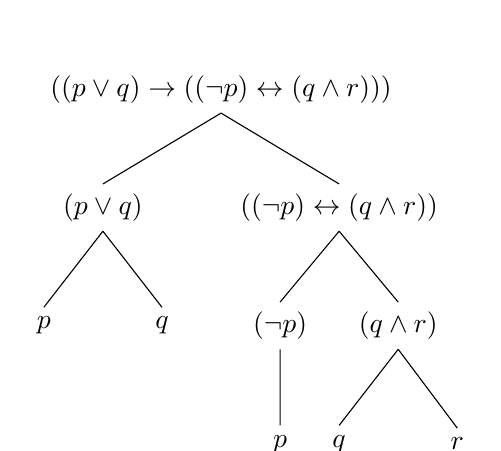
\begin{tikzpicture}[
  level distance=1.5cm,
  level 1/.style={sibling distance=3cm},
  level 2/.style={sibling distance=1.5cm}]
  sibling distance=6cm,
  tlabel/.style={pos=0.4,right=-1pt,font=\footnotesize\color{black}},
]
\node{$((p \vee q) \rightarrow ((\neg p) \leftrightarrow (q \wedge r)))$}
child {node {$(p \vee q)$}
  child {node {$p$}}
  child {node {$q$}}
}
child{node {$((\neg p) \leftrightarrow (q \wedge r))$}
  child {node {$(\neg p)$}
    child {node {$p$}}
  }
  child {node {$(q \wedge r)$}
    child {node {$q$}}
    child {node {$r$}}
  }
};
\end{tikzpicture}
\end{center}

\item $(((\neg p) \wedge q) \rightarrow (p \wedge (q \vee (\neg r))))$
\begin{center}
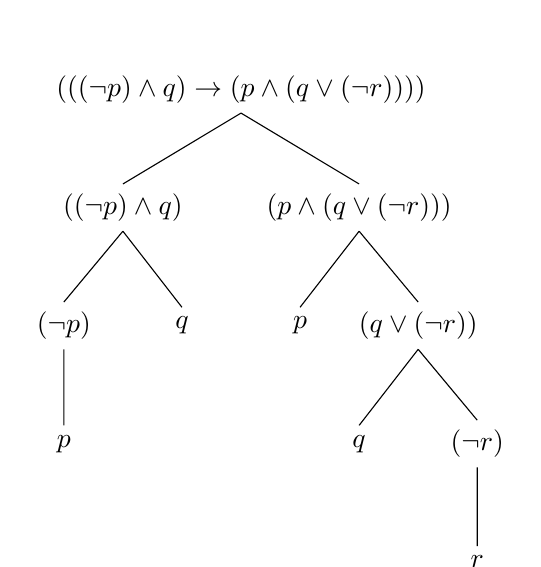
\begin{tikzpicture}[
  level distance=1.5cm,
  level 1/.style={sibling distance=3cm},
  level 2/.style={sibling distance=1.5cm}]
  sibling distance=6cm,
  tlabel/.style={pos=0.4,right=-1pt,font=\footnotesize\color{black}},
]
\node{$(((\neg p) \wedge q) \rightarrow (p \wedge (q \vee (\neg r))))$}
child {node {$((\neg p) \wedge q)$}
  child {node {$(\neg p)$}
    child {node {$p$}}
  }
  child {node {$q$}}
}
child{node {$(p \wedge (q \vee (\neg r)))$}
  child {node {$p$}}
  child {node {$(q \vee (\neg r))$}
    child {node {$q$}}
    child {node {$(\neg r)$} 
      child {node {$r$}}
    }
  }
};
\end{tikzpicture}
\end{center}
\end{enumerate}

\subsection{Precedence Rules}
Consider the following the following sequence of connectives:
$$\neg, \wedge, \vee, \rightarrow, \leftrightarrow$$
Each connective on the left has priority over those on the right.

\newpage
\section{Structural Induction}

\subsection{Unique Readability of Well-Formed Formulas}

\begin{thm}[Unique readability theorem]
There is a unique way to construct each well-formed formula.
\end{thm}

Other properties of well-formed formulas that can be proven: \vspace{-0.25cm}
\begin{itemize}
    \item Every well-formed formula has at least one propositional variable. 
    \item Every well-formed formula has an equal number of opening and closing brackets.
    \item Every proper prefix of a well-formed formula has more opening brackets than closing brackets. 
    \item There is a unique way to construct every well-formed formula.
\end{itemize}

\subsection{Recursive Structure in Well-Formed Formulas}
From the definition of ${\rm Form}(\mathcal{L}^p)$, \vspace{-0.25cm}
\begin{enumerate}
    \item ${\rm Atom}(\mathcal{L}^p) \subseteq {\rm Form}(\mathcal{L}^p)$. (Base case)
    \item If $A \in {\rm Form}(\mathcal{L}^p)$, then $(\neg A) \in {\rm Form}(\mathcal{L}^p)$. (Inductive case)
    \item If $A, B \in {\rm Form}(\mathcal{L}^p)$, then $(A * B) \in {\rm Form}(\mathcal{L}^p)$. (Inductive case)
\end{enumerate}

\subsection{Structural Induction Template for Well-Formed Formulas}
\begin{thm*}
For every well-formed formula $\varphi$, $P(\varphi)$ holds. 
\end{thm*}
\begin{pf} 
Proof by structural induction:

{\bf Base case.} $\varphi$ is a propositional symbol $q$. Prove that $P(q)$ holds.

{\bf Induction step.} 

{\it Case 1.} $\varphi$ is $(\neg a)$, where $a$ is well-formed. \\
Assume $P(a)$ holds. We need to prove that $P((\neg a))$ holds.

{\it Case 2.} $\varphi$ is $(a * b)$ where $a$ and $b$ are well-formed and $*$ is a binary connective. \\
Assume $P(a)$ and $P(b)$ hold. We need to prove that $P((a * b))$ holds.

By the principle of structural induction, $P(\varphi)$ holds for every well-formed formula $\varphi$.
\end{pf}

\begin{exmp}
Prove that every well-formed propositional formula has an equal number of opening and closing brackets.
\end{exmp}
\begin{pf} Define $P(\varphi)$ to be that $\varphi$ has an equal number of opening and closing brackets.

{\bf Base case.} $\varphi$ is a propositional symbol $q$. Since $q$ has zero opening and closing brackets, $P(q)$ holds.

{\bf Induction step.} Let ${\rm op}(a)$ and ${\rm cl}(a)$ denote the number of opening and closing brackets in $a$, respectively.

{\it Case 1.} $\varphi$ is $(\neg a)$ where $a \in {\rm Form}(\mathcal{L}^p)$. 

Suppose that $P(a)$ holds. That is, ${\rm op}(a) = {\rm cl}(a)$. Then we have
\begin{align*}
    {\rm op}((\neg a)) 
    &= 1 + {\rm op}(a) & \text{(by inspection of $(\neg a)$)} \\
    &= 1 + {\rm cl}(a) & \text{(by inductive hypothesis)} \\
    &= {\rm cl}((\neg a)) & \text{(by inspection of $(\neg a)$)}
\end{align*}
Thus, $P((\neg a))$ holds.

{\it Case 2.} $\varphi$ is $(a * b)$ where $a, b \in {\rm Form}(\mathcal{L}^p)$ and $*$ is a binary connective.

Suppose that $P(a)$ and $P(b)$ holds. Hence ${\rm op}(a) = {\rm cl}(a)$ and ${\rm op}(b) = {\rm cl}(b)$. Then
\begin{align*}
{\rm op}((a * b)) 
&= {\rm op}(a) + {\rm op}(b) + 1 & \text{(by construction)} \\
&= {\rm cl}(a) + {\rm cl}(b) + 1 & \text{(by inductive hypothesis)} \\
&= {\rm cl}((a * b)) & \text{(by construction)}
\end{align*}
Hence $P((a * b))$ holds.

By the principle of structural induction, $P(\varphi)$ holds for every well-formed formula $\varphi$.
\end{pf}

\begin{exmp} 
Every proper prefix of a well-formed formula has more opening brackets than closing brackets.
\end{exmp}
\begin{pf} 

Proof by structural induction:

Let $P(\varphi)$ denote the property that every proper prefix of the well-formed formula $\varphi$ has more opening than closing brackets. 

{\bf Base case.} $\varphi$ is a propositional variable $q$.

$q$ has no proper prefix, so $P(q)$ is true.

{\bf Induction step.} Let ${\rm op}(a)$ and ${\rm cl}(a)$ denote the number of opening and closing brackets in $a$, respectively.

{\it Case 1.} $\varphi$ is $(\neg a)$ where $a \in {\rm Form}(\mathcal{L}^p)$.

Suppose that $P(a)$ holds. We need to prove that $P((\neg a))$ is true.

We prove this for two interesting cases: \vspace{-0.25cm}
\begin{enumerate}[(1)]
\item $(\neg m$ -- $m$ is a proper prefix of $a$

We have
\begin{align*}
    {\rm op}((\neg m) 
    &= {\rm op}(m) + 1 \\
    &> {\rm cl}(m) \\
    &= {\rm cl}((\neg m)
\end{align*}

\item $(\neg a$

Observe that
\begin{align*}
    {\rm op}((\neg a) 
    &= 1 + {\rm op}(a) \\
    &> 1 + {\rm cl}(a) \\
    &= {\rm cl}((\neg a)
\end{align*}
\end{enumerate}
There are other cases -- to be completed.
\end{pf}

Structural induction is an important concept that does not only apply to well-formed formulas. 

\subsection{Defining Sets Inductively}
An inductive definition of a set consists of three components: \vspace{-0.25cm}
\begin{itemize}
    \item A domain set $X$
    \item A core set $C$
    \item A set of operations of $P$
\end{itemize}
\vspace{-0.25cm}
Given a domain set $X$, a core set $C$, and a set of operations $P$, $I(X, C, P)$ is the minimal subset of $X$ that contains $C$ and is closed under $P$.

\begin{defn}[Closed]
A set $Y$ is {\bf closed under a set of operations $P$} if and only if applying any operation in $P$ to elements in $Y$ will always return an element in $Y$.
\end{defn}

\begin{defn}[Minimal set]
A set $Y$ is a {\bf minimal set with respect to a property $R$} if \vspace{-0.25cm}
\begin{itemize}
    \item $Y$ has property $R$, and
    \item for every set $Z$ that has property $R$, we have $Y \subseteq Z$.
\end{itemize}
\end{defn}

We can define the set of well-formed formulas inductively. 
\begin{align*}
    X &: \text{any finite sequence of symbols of } \mathcal{L}^p \\
    C &: \text{propositional symbols, e.g. } p, q, r \\
    P &: f(a) = (\neg a) \text{ and } f(a, b) = (a * b) \text{ where } * \text{ is one of } \wedge, \vee, \rightarrow, \leftrightarrow
\end{align*}

\subsection{Structural Induction on $I(X, C, P)$}
{\bf Claim.} Every element of the set $I(X, C, P)$ has the property $R$.
\begin{pf} Proof by structural induction:

{\bf Base case.} Prove that $R$ holds for every element in the core set $C$.

{\bf Inductive case.} Prove that for every operation $f \in P$ of arity $k$ and any $y_1, \dots, y_k \in I(X, C, P)$ such that $R(y_1), \dots, R(y_k)$, $R(f(y_1, \dots, y_k))$ holds.
\end{pf}

\begin{exmp}
Let $X = \R$, $C = \{0, 2\}$, and $P = \{f_1(x, y) = x + y, f_2(x, y) = x - y\}$. Show that every element of $I(X, C, P)$ is an even integer.
\end{exmp} 
\begin{pf}~

{\bf Base case.} 0 and 2 are both even.

{\bf Inductive case.} Assume that $a$ and $b$ are even integers where $a, b \in I(X, C, P)$. We have $a = 2m$ for some $m \in \Z$, and $b = 2n$ for some $n \in \Z$ by hypothesis. Hence $a + b = 2(m+n)$ for $m + n \in \Z$ and $a - b = 2(m - n)$ for $m - n \in \Z$, so we are done.
\end{pf}

\newpage
\section{Semantics}

\subsection{Truth Valuation}

\begin{defn}[Truth valuation]
A {\bf truth valuation} is a function with the set of all propositional symbols as the domain and $\{1, 0\}$ as the range.

We use $t$ to denote any truth valuation.

The value which $t$ assigns to any formula $A$ is written as $A^t$.
\end{defn}

\subsection{Proving or Disproving an Implication}
Let $A$ and $B$ be well-formed propositional formulas. Consider $A \rightarrow B$. 

To prove an implication is false, we need to find a truth valuation $t$ such that $A^t = 1$ and $B^t = 0$.

To prove an implication is true, show that for every truth valuation $t$ such that $A^t = 1$, we have $B^t = 1$. 

\subsection{Tautology, Contradiction, Satisfiable}

\begin{defn}
A formula $A$ is a {\bf tautology} if and only if for every truth valuation $t$, $A^t = 1$.

A formula $A$ is a {\bf contradiction} if and only if for every truth valuation $t$, $A^t = 0$.

A formula $A$ is {\bf satistiable} if and only if there exists a truth valuation $t$ such that $A^t = 1$.
\end{defn}

To determine if a formula is a tautology, a contradiction, or satisfiable, we have three approaches: \vspace{-0.25cm}
\begin{itemize}
    \item Draw a truth table.
    \item Draw a valuation tree (a more compact truth table).
    \item Use reasoning to get an answer quickly.
\end{itemize}
\vspace{-0.25cm}

After plugging in a formula, we can simplify a formula as follows:
\begin{align*}
    \begin{aligned}
    p \wedge 1 & \equiv p \\
    p \wedge 0 & \equiv 0 \\
    p \wedge p & \equiv p \\
    \end{aligned}
    & &
    \begin{aligned}
    p \vee 1 & \equiv 1 \\
    p \vee 0 & \equiv p \\
    p \vee p & \equiv p \\
    \end{aligned}
    & & 
    \begin{aligned}
    p \rightarrow 1 & \equiv 1 \\
    p \rightarrow 0 & \equiv (\neg p) \\
    1 \rightarrow p & \equiv p \\
    0 \rightarrow p & \equiv 1 \\
    p \rightarrow p & \equiv 1 \\
    \end{aligned}
    & & 
    \begin{aligned}
    p \leftrightarrow 1 & \equiv p \\
    p \leftrightarrow 0 & \equiv (\neg p) \\
    p \leftrightarrow p & \equiv 1 \\
    \end{aligned}
\end{align*}

\newpage
\subsection{Valuation Trees}
\begin{exmp}
Prove that $(((p \wedge q) \rightarrow (\neg r)) \wedge (p \rightarrow q)) \rightarrow (p \rightarrow (\neg r))$ is a tautology.

\begin{center}
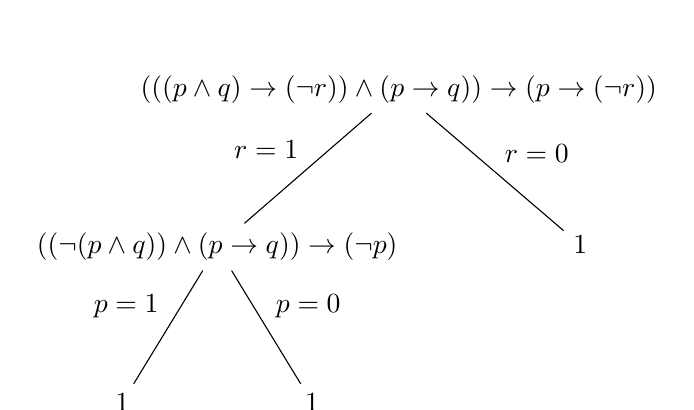
\begin{tikzpicture}[
  level distance=2cm,sibling distance=2cm,
  edge from parent path={(\tikzparentnode) -- (\tikzchildnode)}]
\Tree
[.{$(((p \wedge q) \rightarrow (\neg r)) \wedge (p \rightarrow q)) \rightarrow (p \rightarrow (\neg r))$}
  \edge node[auto=right] {$r = 1$};
  [.{$((\neg (p \wedge q)) \wedge (p \rightarrow q)) \rightarrow (\neg p)$}
    \edge node[auto=right] {$p = 1$};
    [.1 ]
    \edge node[auto=left] {$p = 0$};
    [.1 ]
  ]
  \edge node[auto=left] {$r = 0$};
  [.1 ]
]
\end{tikzpicture}
\end{center}

Hence, the formula is a tautology.
\end{exmp}

\begin{exmp}
Determine if the formula $((p \vee q) \leftrightarrow ((p \wedge (\neg q)) \vee ((\neg p) \wedge q)))$ is a tautology, a contradiction, or satisfiable but not a tautology using a valuation tree.

\begin{center}
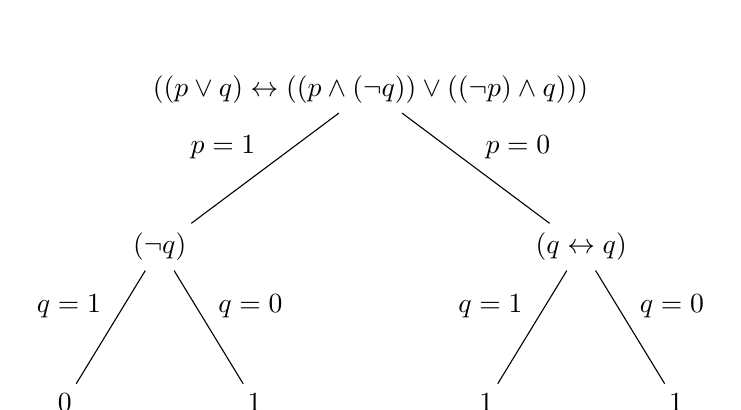
\begin{tikzpicture}[
  level distance=2cm,sibling distance=2cm,
  edge from parent path={(\tikzparentnode) -- (\tikzchildnode)}]
\Tree
[.{$((p \vee q) \leftrightarrow ((p \wedge (\neg q)) \vee ((\neg p) \wedge q)))$}
  \edge node[auto=right] {$p = 1$};
  [.{$(\neg q)$}
    \edge node[auto=right] {$q = 1$};
    [.0 ]
    \edge node[auto=left] {$q = 0$};
    [.1 ]
  ]
  \edge node[auto=left] {$p = 0$};
  [.{$(q \leftrightarrow q)$}
    \edge node[auto=right] {$q = 1$};
    [.1 ]
    \edge node[auto=left] {$q = 0$};
    [.1 ]
    ]
  ]
]
\end{tikzpicture}
\end{center}

Thus the formula is satisfiable but not a tautology.

(Note: This asks if an inclusive or is equivalent to an exclusive or.)
\end{exmp}

\newpage
\section{Tautological Consequence and Translations}
\subsection{Satisfying a Set of Formulas}
Let $\Sigma^t$ denote any set of formulas.
$$\Sigma^t = \begin{cases} 1, \text{ if for each } B \in \Sigma, B^t = 1 \\ 0, \text{ otherwise} \end{cases}$$

\begin{defn}[Satisfiability]
We say that $\Sigma$ is {\bf satisfiable} if and only if there is some truth valuation $t$ such that $\Sigma^t = 1$. When $\Sigma^t = 1$, $t$ is said to satisfy $\Sigma$.
\end{defn}

\subsection{Tautological Consequence}

\begin{defn}[Tautological consequence]
Suppose $\Sigma \subseteq {\rm Form}(\mathcal{L}^p)$ and $A \in {\rm Form}(\mathcal{L}^p)$. 

$A$ is a {\bf tautological consequence} of $\Sigma$ (that is, of the formulas in $\Sigma$), written as $\Sigma \vDash A$, if and only if for every truth valuation $t$, $\Sigma^t = 1$ implies $A^t = 1$.
\end{defn}

\begin{defn}[Tautological equivalence]
$A$ and $B$ are (tautologically) equivalent if and only if $A \vDashv B$ holds, where $A \vDashv B$ denotes $A \vDash B$ and $B \vDash A$. 
\end{defn}

\begin{exercise} 
Show that $\{(\neg (p \wedge q)), (p \rightarrow q)\} \vDash (\neg p)$.
\end{exercise}
\begin{pf}
Consider any truth valuation $t$ such that $(\neg (p \wedge q))^t = 1$ and $(p \rightarrow q)^t = 1$. We want to prove that $(\neg p)^t = 1$. 

Since $(\neg (p \wedge q))^t = 1$, we have $(p \wedge q)^t = 0$ by the truth table of $\neg$. By the truth table of $\wedge$, there are three possible cases: 

\begin{center}
\begin{enumerate*}[(1)]
\item $p^t = 0$, $q^t = 1$ \quad
\item $p^t = 1$, $q^t = 0$ \quad
\item $p^t = q^t = 0$
\end{enumerate*}
\end{center}

Since $(p \rightarrow q)^t = 1$, it is impossible that $p^t = 1$ and $q^t = 0$ by the truth table of $\rightarrow$. This leaves the cases (1) and (3). In both these cases, $p^t = 0$ and hence $(\neg p)^t = 1$ by the truth table of $\neg$.
\end{pf}

\begin{exercise}
Show that $\{(\neg (p \wedge q)), (p \rightarrow q)\} \nvDash (p \leftrightarrow q)$.
\end{exercise}
\begin{pf}
We need to find a truth valuation $t$ such that $(\neg (p \wedge q))^t = 1$, $(p \rightarrow q)^t = 1$, and $(p \leftrightarrow q)^t = 0$. 

Consider the truth valuation $t$ with $p^t = 0$, $q^t = 1$.

We have $(p \wedge q)^t = 0$ by the truth table of $\wedge$, and $(\neg (p \wedge q))^t = 1$ by the truth table of $\neg$. 
Also, $(p \rightarrow q)^t = 1$ by the truth table of $\rightarrow$, and $(p \leftrightarrow q)^t = 0$ by the truth table of $\leftrightarrow$.
\end{pf}

\subsection{Translations}
Translating English sentences to propositional formulas:

$\neg p$: $p$ does not hold; $p$ is false; it is not the case that $p$

$p \wedge q$: $p$ but $q$; not only $p$ but $q$; $p$ while $q$; $p$ despite $q$; $p$ yet $q$; $p$ although $q$

$p \vee q$: $p$ or $q$ or both; $p$ and/or $q$

$p \rightarrow q$: $p$ implies $q$; $q$ if $p$; $p$ only if $q$; $q$ when $p$; $p$ is sufficient for $q$; $q$ is necessary for $p$

$p \leftrightarrow q$: $p$ is equivalent to $q$; $p$ exactly if $q$; $p$ is necessary and sufficient for $q$

\newpage
\section{Formal Deduction}

\subsection{Formal Deducibility}
Let the relation of formal deducibility be denoted by
$$\Sigma \vdash A,$$
which means that $A$ is formally deducible (or provable) from $\Sigma$.

\subsection{Rules of Formal Deduction}
Refer to pages 29 and 30 of \href{https://cs.uwaterloo.ca/~a23gao/cs245_f19/notes/workbook_sol.pdf}{this pdf}.
%{\bf Set membership ($\in$):} If $A \in \Sigma$, then $\Sigma \vdash A$.

%{\bf Reflexivity (Ref):} $A \vdash A$.

%{\bf Addition of premises (+):} If $\Sigma \vdash A$, then $\Sigma, \Sigma' \vdash A$.

%{\bf And introduction ($\wedge+$):} If $\Sigma \vdash A$, $\Sigma \vdash B$, then $\Sigma \vdash A \wedge B$.

%{\bf And elimination ($\wedge-$):} If $\Sigma \vdash A \wedge B$, then $\Sigma \vdash A$. If $\Sigma \vdash A \wedge B$, then $\Sigma \vdash B$.

%{\bf Or introduction ($\vee+$):} If $\Sigma \vdash A$, then $\Sigma \vdash A \vee B$. If $\Sigma \vdash B$, then $\Sigma \vdash A \vee B$.

%{\bf Or elimination ($\vee-$):} If $\Sigma, A \vdash C$, $\Sigma, B \vdash C$, then $\Sigma, A \vee B \vdash C$.

%{\bf Negation introduction ($\neg+$):} If $\Sigma, A \vdash B$, $\Sigma, A \vdash \neg B$, then $\Sigma \vdash \neg A$.

%{\bf Negation elimination ($\neg-$):} If $\Sigma, \neg A \vdash B$, $\Sigma, \neg A \vdash \neg B$, then $\Sigma \vdash A$.

%{\bf Implication introduction ($\rightarrow+$):} If $\Sigma, A \vdash B$, then $\Sigma \vdash A \rightarrow B$.

%{\bf Implication elimination ($\rightarrow-$):} If $\Sigma \vdash A$, $\Sigma \vdash A \rightarrow B$, then $\Sigma \vdash B$.

%{\bf Equivalence introduction ($\leftrightarrow+$):} If $\Sigma, A \vdash B$, $\Sigma, B \vdash A$, then $\Sigma \vdash A \leftrightarrow B$.

%{\bf Equivalence elimination ($\leftrightarrow-$):} If $\Sigma \vdash A$, $\Sigma \vdash A \leftrightarrow B$, then $\Sigma \vdash B$. \\ If $\Sigma \vdash B$, $\Sigma \vdash A \leftrightarrow B$, then $\Sigma \vdash A$. 

\subsection{Formal Deduction Examples}

\begin{exercise}
Show that $\{(p \wedge q), (r \wedge s)\} \vdash (q \wedge s)$.

Solution:
\begin{align*}
    (1) & & p \wedge q,\, r \wedge s &\vdash p \wedge q & & \text{by ($\in$)} \\
    (2) & & p \wedge q,\, r \wedge s &\vdash q & & \text{by ($\wedge-$, 1)} \\
    (3) & & p \wedge q,\, r \wedge s &\vdash r \wedge s & & \text{by ($\in$)} \\
    (4) & & p \wedge q,\, r \wedge s &\vdash s & & \text{by ($\wedge-$, 3)} \\
    (5) & & p \wedge q,\, r \wedge s &\vdash q \wedge s & & \text{by ($\wedge+$, 2, 4)}
\end{align*}
\end{exercise}

\begin{exercise}
Show that $\{(p \rightarrow q), (q \rightarrow r)\} \vdash (p \rightarrow r)$.

Solution:
\begin{align*}
    (1) & & p \rightarrow q,\, q \rightarrow r,\, p &\vdash p & & \text{by ($\in$)} \\
    (2) & & p \rightarrow q,\, q \rightarrow r,\, p &\vdash p \rightarrow q & & \text{by ($\in$)} \\
    (3) & & p \rightarrow q,\, q \rightarrow r,\, p &\vdash q & & \text{by ($\rightarrow-$, 1, 2)} \\
    (4) & & p \rightarrow q,\, q \rightarrow r,\, p &\vdash q \rightarrow r & & \text{by ($\in$)} \\
    (5) & & p \rightarrow q,\, q \rightarrow r,\, p &\vdash r & & \text{by ($\rightarrow-$, 3, 4)} \\
    (6) & & p \rightarrow q,\, q \rightarrow r &\vdash p \rightarrow r & & \text{by ($\rightarrow+$, 5)} \\
\end{align*}
\end{exercise}

\newpage
\begin{exercise}
Show that $\{(p \vee q)\} \vdash ((p \rightarrow q) \vee (q \rightarrow p))$. 

Solution:
\begin{align*}
    (1) & & p,\, q &\vdash p & & \text{by ($\in$)} \\
    (2) & & p,\, q &\vdash q & & \text{by ($\in$)} \\
    (3) & & p &\vdash q \rightarrow p & & \text{by ($\rightarrow+$, 1)} \\
    (4) & & q &\vdash p \rightarrow q & & \text{by ($\rightarrow+$, 2)} \\
    (5) & & p &\vdash (p \rightarrow q) \vee (q \rightarrow p) & & \text{by ($\vee+$, 3)} \\
    (6) & & q &\vdash (p \rightarrow q) \vee (q \rightarrow p) & & \text{by ($\vee+$, 4)} \\
    (7) & & p \vee q &\vdash (p \rightarrow q) \vee (q \rightarrow p) & & \text{by ($\vee+$, 5, 6)} \\
\end{align*}
\end{exercise}

\begin{exercise}
Show that $\{(p \rightarrow (q \rightarrow r)), (p \rightarrow q)\} \vdash (p \rightarrow r)$.

Solution:
\begin{align*}
    (1) & & p \rightarrow (q \rightarrow r),\, p \rightarrow q,\, p  &\vdash p & & \text{by ($\in$)} \\
    (2) & & p \rightarrow (q \rightarrow r),\, p \rightarrow q,\, p  &\vdash p \rightarrow q & & \text{by ($\in$)} \\
    (3) & & p \rightarrow (q \rightarrow r),\, p \rightarrow q,\, p  &\vdash q & & \text{by ($\rightarrow-$, 1, 2)} \\
    (4) & & p \rightarrow (q \rightarrow r),\, p \rightarrow q,\, p  &\vdash p \rightarrow (q \rightarrow r) & & \text{by ($\in$)} \\
    (5) & & p \rightarrow (q \rightarrow r),\, p \rightarrow q,\, p  &\vdash q \rightarrow r & & \text{by ($\rightarrow-$, 1, 4)} \\
    (6) & & p \rightarrow (q \rightarrow r),\, p \rightarrow q,\, p  &\vdash r & & \text{by ($\rightarrow-$, 3, 5)} \\
    (7) & & p \rightarrow (q \rightarrow r),\, p \rightarrow q &\vdash p \rightarrow r & & \text{by ($\rightarrow+$, 6)} \\
\end{align*}
\end{exercise}

\begin{exercise}
Show that $\{(p \rightarrow q)\} \vdash (r \vee p) \rightarrow (r \vee q)$. 

Solution:
\begin{align*}
    (1) & & p \rightarrow q,\, r &\vdash r & & \text{by ($\in$)} \\
    (2) & & p \rightarrow q,\, r &\vdash r \vee q & & \text{by ($\vee+$, 1)} \\
    (3) & & p \rightarrow q,\, p &\vdash p & & \text{by ($\in$)} \\
    (4) & & p \rightarrow q,\, p &\vdash p \rightarrow q & & \text{by ($\in$)} \\
    (5) & & p \rightarrow q,\, p &\vdash q & & \text{by ($\rightarrow-$, 3, 4)} \\
    (6) & & p \rightarrow q,\, p &\vdash r \vee q & & \text{by ($\vee+$, 5)} \\
    (7) & & p \rightarrow q,\, r \vee p &\vdash r \vee q & & \text{by ($\vee-$, 2, 6)} \\
    (8) & & p \rightarrow q &\vdash (r \vee p) \rightarrow (r \vee q) & & \text{by ($\rightarrow+$, 7)} 
\end{align*}
\end{exercise}

\newpage
\begin{exercise}
Show that $\{(p \rightarrow (q \rightarrow r)),\, p,\, (\neg r)\} \vdash (\neg q)$.

Solution:
\begin{align*}
    (1) & & p \rightarrow (q \rightarrow r),\, p,\, (\neg r), q &\vdash p & & \text{by ($\in$)} \\
    (2) & & p \rightarrow (q \rightarrow r),\, p,\, (\neg r), q &\vdash q & & \text{by ($\in$)} \\
    (3) & & p \rightarrow (q \rightarrow r),\, p,\, (\neg r), q &\vdash p \rightarrow (q \rightarrow r) & & \text{by ($\in$)} \\
    (4) & & p \rightarrow (q \rightarrow r),\, p,\, (\neg r), q &\vdash q \rightarrow r & & \text{by ($\rightarrow-$, 1, 3)} \\
    (5) & & p \rightarrow (q \rightarrow r),\, p,\, (\neg r), q &\vdash r & & \text{by ($\rightarrow-$, 2, 4)} \\
    (6) & & p \rightarrow (q \rightarrow r),\, p,\, (\neg r), q &\vdash (\neg r)  & & \text{by ($\in$)} \\
    (7) & & p \rightarrow (q \rightarrow r),\, p,\, (\neg r) &\vdash (\neg q) & & \text{by ($\neg+$, 5, 6)} 
\end{align*}
\end{exercise}

\newpage
\section{Soundness of Formal Deduction}

\subsection{Tautological Consequence v.s. Formal Deduction}
$\Sigma \vDash A$ and $\Sigma \vdash A$ appear to be similar. Ideally, we would like them to be equivalent. This could mean two properties: \vspace{-0.25cm}
\begin{enumerate}
    \item If $\Sigma \vdash A$, then $\Sigma \vDash A$. [Soundness of formal deduction] \\
    If there exists a formal proof from $\Sigma$ to $A$, then $\Sigma$ tautologically implies $A$.
    \item If $\Sigma \vDash A$, then $\Sigma \vdash A$. [Completeness of formal deduction] \\
    If $\Sigma$ tautologically implies $A$, there exists a formal proof from $\Sigma$ to $A$.
\end{enumerate}

\begin{thm}
Formal deduction is both sound and complete.
\end{thm}

\subsection{Proving the Soundness of Formal Deduction}
We will prove this by structural induction on the proof for $\Sigma \vdash A$. Note that the proof is a recursive structure.

\begin{thm}[Soundness Theorem]
For a set of propositional formulas $\Sigma$ and a propositional formula $A$, we have that $\Sigma \vdash A$ implies $\Sigma \vDash A$.
\end{thm}
\begin{pf}
We prove this by structural induction on the proof for $\Sigma \vdash A$.

{\sc Base case.} Assume that there is a proof for $\Sigma \vdash A$ where $A \in \Sigma$. Consider a truth valuation such that $\Sigma^t = 1$. Since $A \in \Sigma$, then $A^t = 1$. Thus, $\Sigma \vDash A$.

{\sc Induction step.} Consider several cases for the last rule applied in the proof of $\Sigma \vdash A$.

{\bf Case 1.} Assume that the proof of $\Sigma \vdash A$ applies the rule $\wedge+$ with the two premises $\Sigma \vdash B$ and $\Sigma \vdash C$ and reaches the conclusion $\Sigma \vdash B \wedge C$.

{\bf Induction hypothesis.} Assume that $\Sigma \vDash B$ and $\Sigma \vDash C$. We need to prove that $\Sigma \vDash B \wedge C$.

Consider any truth valuation $t$ such that $\Sigma^t = 1$. By the induction hypothesis, we have that $B^t = C^t = 1$. By the truth table of $\wedge$, $(B \wedge C)^t = 1$, therefore $\Sigma \vDash B \wedge C$.

{\bf Case 2.} Assume that the proof of $\Sigma \vdash A$ applies the rule $\rightarrow-$ with the two premises $\Sigma \vdash B$ and $\Sigma \vdash (B \rightarrow C)$ and reaches the conclusion $\Sigma \vdash C$.

{\bf Induction hypothesis.} Assume that $\Sigma \vDash B$ and $\Sigma \vDash (B \rightarrow C)$. We need to show that $\Sigma \vDash C$.

Consider any truth valuation $t$ such that $\Sigma^t - 1$. By the induction hypothesis, we have that $B^t = 1$ and $(B \rightarrow C)^t = 1$. By the truth table of $\rightarrow$, we have that $C^t = 1$, therefore $\Sigma \vDash C$.

The other 10 cases (formal deduction rules) are similar.
\end{pf}

\newpage
\subsection{Applications of Soundness and Completeness}

\begin{enumerate}

\item The following inference rule is called disjunctive syllogism:
\begin{center}
    If $\Sigma \vdash \neg A$ and $\Sigma \vdash A \vee B$, then $\Sigma \vdash B$.
\end{center}
where $A$ and $B$ are well-formed propositional formulas.

Prove that this inference rule is sound. That is, prove that if $\Sigma \vDash \neg A$ and $\Sigma \vDash A \vee B$, then $\Sigma \vDash B$.

\begin{pf}
Assume $\Sigma \vDash \neg A$ and $\Sigma \vDash A \vee B$. We need to show that $\Sigma \vDash B$. 

Consider a truth valuation $t$ such that $\Sigma^t = 1$. Since $\Sigma \vDash \neg A$, we have $(\neg A)^t = 1$. By the truth table of $\neg$, $A^t = 0$. Since $\Sigma \vDash A \vee B$, at least one of $A^t = 1$ and $B^t = 1$ by the truth table of $\vee$. Since $A^t = 0$, we must have $B^t = 1$. Therefore, $\Sigma \vDash B$.
\end{pf}

\item Show that there does not exist a formal deduction proof for $p \vee q \vdash p$, where $p$ and $q$ are propositional variables.

\begin{pf}
By the contrapositive of the soundness of formal deduction, if $p \vee q \nvDash p$, then $p \vee q \nvdash p$; that is, there does not exist a formal proof for $p \vee q \vdash p$. 

We show that $p \vee q \nvDash p$. Consider a truth valuation $t$ such that $p^t = 0$ and $q^t = 1$. Then $(p \vee q)^t = 1$ by the truth table by $\vee$, but $p^t = 0$, hence we have $p \vee q \nvDash p$. This implies that $p \vee q \nvdash p$, as required.
\end{pf}

\item Prove that $(A \rightarrow B) \nvdash (B \rightarrow A)$ where $A$ and $B$ are propositional formulas.

\begin{pf}
By the contrapositive of the soundness of formal deduction, if $(A \rightarrow B) \nvDash (B \rightarrow A)$, then $(A \rightarrow B) \nvdash (B \rightarrow A)$. We need to give a counter example to show that $(A \rightarrow B) \nvDash (B \rightarrow A)$. 

Let $A = p$ and $B = q$. Consider the truth valuation where $p^t = 0$ and $q^t = 1$. By the truth table of $\rightarrow$, $(p \rightarrow q)^t = 1$ and $(q \rightarrow p)^t = 0$. Therefore, $(A \rightarrow B) \nvDash (B \rightarrow A)$, and thus, $(A \rightarrow B) \nvdash (B \rightarrow A)$.
\end{pf}

\end{enumerate}

\newpage
\section{Completeness of Formal Deduction}

\subsection{The Completeness Theorem}
\begin{thm}
If $\Sigma \vDash A$, then $\Sigma \vdash A$.

{\bf Proof Sketch.}

If $\Sigma$ is consistent implies that $\Sigma$ is satisfiable, then $\Sigma \vDash A$ implies $\Sigma \vdash A$ (done in lecture). 

If $\Sigma \vDash A$ implies $\Sigma \vdash A$, then $\Sigma$ is consistent implies that $\Sigma$ is satisfiable (on the assignment). 
\vspace{-1cm}
\begin{flushright} $\qed$ \end{flushright}
\end{thm}
\vspace{-0.25cm}

\subsection{Satisfiable and Consistent}
Recall that $\Sigma$ is satisfiable if there exists a truth valuation $t$ such that for every $A \in \Sigma$, $A^t = 1$.

\begin{defn}[Consistent]
Intuitively, $\Sigma$ is consistent if it doesn't prove a contradiction.

Two equivalent definitions: \vspace{-0.25cm}
\begin{itemize}
    \item There exists a formula $A$ such that $\Sigma \nvdash A$.
    \item For every formula $A$, if $\Sigma \vdash A$, then $\Sigma \nvdash (\neg A)$.
\end{itemize}
\vspace{-0.25cm}
Note that consistency is a syntactical notion.
\end{defn}
\vspace{-.25cm}
We will prove that these two definitions are equivalent.

{\bf Proof.}

(2) $\rightarrow$ (1). Assume that for every formula $A$, $\Sigma \vdash A$ implies that $\Sigma \nvdash (\neg A)$. We need to find a formula $A$ such that $\Sigma \nvdash A$. 

Choose any propositional formula $A$. If $\Sigma \nvdash A$, we are done. If $\Sigma \vdash A$, by our assumption, we have that $\Sigma \nvdash (\neg A)$. Thus, $(\neg A)$ is the formula we require, so we are done.

(1) $\rightarrow$ (2). We prove the contrapositive. Assume that there exists a formula $A$ such that $\Sigma \vdash A$ and $\Sigma \vdash (\neg A)$. We need to prove that for every formula $B$, $\Sigma \vdash B$. 

Let $B$ be any formula. Then
\begin{align*}
    (1) & & \Sigma &\vdash A & & \text{by assumption} \\
    (2) & & \Sigma,\, \neg B &\vdash A & & \text{by ($+$, 1)} \\
    (3) & & \Sigma &\vdash \neg A & & \text{by assumption} \\
    (4) & & \Sigma,\, \neg B &\vdash \neg A & & \text{by ($+$, 3)} \\
    (5) & & \Sigma &\vdash B & & \text{by ($\neg-$, 2, 4)} 
\end{align*}
Thus $\Sigma \vdash B$ for every formula $B$.
\vspace{-1cm} \begin{flushright} $\qed$ \end{flushright}

\subsection{Proving the Completeness Theorem}
We prove one direction: if $\Sigma$ is consistent implies that $\Sigma$ is satisfiable, then $\Sigma \vDash A$ implies $\Sigma \vdash A$. 

{\bf Proof.} Assume that $\Sigma \vDash A$.

If $\Sigma \vDash A$, then we can prove that $\Sigma \cup \{\neg A\}$ is not satisfiable (on Assignment 4).

Thus, $\Sigma \cup \{\neg A\}$ is not consistent. From this, we will prove that $\Sigma \vdash A$. 

There exists a formula $B$ such that $\Sigma \cup \{\neg A\} \vdash B$ and $\Sigma \cup \{\neg A\} \vdash \neg B$. Then
\begin{align*}
    (1) & & \Sigma,\, \neg A &\vdash B & & \text{by assumption} \\
    (2) & & \Sigma,\, \neg A &\vdash \neg B & & \text{by assumption} \\
    (3) & & \Sigma &\vdash A & & \text{by ($\neg-$, 1, 2)} 
\end{align*}
The other direction is on the assignment.
\vspace{-1cm} \begin{flushright} $\qed$ \end{flushright}

\begin{defn}[Maximally Consistent]
Given a consistent $\Sigma$, $\Sigma$ is maximally consistent if and only if \vspace{-0.25cm}
\begin{itemize}
    \item For every formula $A$, if $\Sigma \nvdash A$, then $\Sigma \cup \{A\}$ is inconsistent.
    \item For every formula $A$, either $\Sigma \vdash A$ or $\Sigma \vdash (\neg A)$, but not both.
\end{itemize}
\vspace{-0.25cm}
These two definitions are equivalent (this is on the assignment).
\end{defn}

{\bf Extending to Maximal Consistency}

Let $\Sigma$ be a consistent set of formulas. $\Sigma$ can be extended to a maximally consistent set $\Sigma^*$ as follows.

Arbitrarily enumerate all the well-formed formulas using the following sequence:
$$A_1, A_2, A_3, \dots$$
Construct an infinite sequence of sets $\Sigma_n$ as follows.
$$\begin{cases} \Sigma_0 = \Sigma \\
\Sigma_{n+1} = \begin{cases} \Sigma_n \cup \{A_{n+1}\}, \text{ if } \Sigma_n \cup \{A_{n+1}\} \text{ is consistent} \\ \Sigma_n, \text{ otherwise} \end{cases} \end{cases}$$

Observe that $\Sigma_n \subseteq \Sigma_{n+1}$ and $\Sigma_n$ is consistent. (We can prove this by induction on $n$.)

Define $\Sigma^* = \cup_{n\in\N} \Sigma_n$. We show that $\Sigma^*$ is the largest possible set that is consistent.

{\bf Consistent.} Suppose to the contrary that $\Sigma^*$ is inconsistent. There is a finite subset $\{B_1, \dots, B_k\} \subseteq \Sigma^*$ which is inconsistent. Suppose that $B_1 \in \Sigma_{i_1},\, \dots,\, B_k \in \Sigma_{i_k}$, and $i = \max(i_1, \dots, i_k)$. By the construction of $\Sigma_n$, we have $\{B_1, \dots, B_k\} \subseteq \Sigma_i$. Then, $\Sigma_i$ is inconsistent, which contradicts the construction of $\Sigma_i$. Hence $\Sigma^*$ must be consistent. 

{\bf Maximally consistent.} Assume that $B$ is a well-formed formula and $\Sigma^* \nvdash B$. We need to show that $\Sigma^* \cup \{B\}$ is inconsistent. Since $\Sigma^* \nvdash B$, it must be that $B \notin \Sigma^*$. $B$ must be in the sequence $A_1, A_2, \dots$. Let $B = A_{m+1}$. By the construction of $\Sigma_n$, $\Sigma_m \cup \{A_{m+1}\}$ is inconsistent. Then, $\Sigma^* \cup \{B\}$ is inconsistent because $\Sigma_m \subseteq \Sigma^*$. Therefore, $\Sigma^*$ is maximally consistent. \hspace{3.5cm} $\qed$

\begin{lemma}
Suppose that $\Sigma$ is maximally consistent. Then $A \in \Sigma$ if and only if $\Sigma \vdash A$.
\end{lemma}

\begin{lemma}
Let $\Sigma^*$ be a maximally consistent set. Let $t$ be a truth valuation such that for every propositional variable $p$, $p^t$ if and only if $p \in \Sigma^*$. 

It follows that for every well-formed propositional formula $A$, $A^t$ if and only if $A \in \Sigma^*$.

{\bf Proof.} 

{\sc Base case.} $A$ is a propositional variable $p$.

By the definition of $t$, $p \in \Sigma$ if and only if $p^t = 1$.

{\sc Inductive step.}

{\bf Inductive case 1.}

{\bf Inductive case 2.} $A$ is $B \wedge C$ for two well-formed formulas $B$ and $C$.

{\small Induction hypothesis.} Assume that $B^t = 1$ if and only if $B \in \Sigma^*$, and $C^t = 1$ if and only if $C \in \Sigma^*$. 

We will show that $(B \wedge C)^t = 1$ if and only if $B \wedge C \in \Sigma^*$.

($\rightarrow$) Assume that $(B \wedge C)^t = 1$. Then $B^t = C^t = 1$ by the truth table of $\wedge$. By the induction hypothesis, $B \in \Sigma^*$ and $C \in \Sigma^*$. By Lemma 8.4, $\Sigma^* \vdash B$ and $\Sigma^* \vdash C$. By ($\wedge+$), $\Sigma^* \vdash B \wedge C$. By Lemma 8.4, $B \wedge C \in \Sigma^*$. 

($\leftarrow$) Assume $B \wedge C \in \Sigma^*$. By Lemma 8.4, $\Sigma^* \vdash B \wedge C$. By ($\wedge-$), $\Sigma^* \vdash B$ and $\Sigma^* \vdash C$. By Lemma 8.4, $B \in \Sigma^*$ and $C \in \Sigma^*$. By the induction hypothesis, $B^t = C^t = 1$, so $(B \wedge C)^t = 1$ by the truth table of $\wedge$.
\vspace{-1cm} \begin{flushright} $\qed$ \end{flushright}
\end{lemma}

\begin{thm}
If $\Sigma$ is consistent, then $\Sigma$ is satisfiable.

{\bf Proof.} Assume that $\Sigma$ is consistent. We need to find a truth valuation $t$ such that $A^t = 1$ for every formula $A \in \Sigma$. 

Extend $\Sigma$ to some maximally consistent set $\Sigma^*$. Let $t$ be a truth valuation such that for every propositional variable $p$, $p^t = 1$ if and only if $p \in \Sigma^*$. 

For every $A \in \Sigma$, $A \in \Sigma^*$. We can prove that $A^t = 1$. Therefore, $\Sigma$ is satisfied by $t$.
\vspace{-1cm} \begin{flushright} $\qed$ \end{flushright}
\end{thm}

\newpage
\section{Predicate Logic}
\subsection{Domains}
A domain is \vspace{-0.25cm}
\begin{itemize}
    \item a non-empty set of objects/individuals.
    \item a word that our statement is situated within.
\end{itemize}
\vspace{-0.25cm}
A statement can have different truth values in different domains.

\subsection{Predicates}
A predicate represents \vspace{-0.25cm}
\begin{itemize}
    \item a property of an individual, or a relationship among multiple individuals.
    \item an $n$-ary function which takes constants and/or variables as inputs and outputs 1 and 0.
\end{itemize}
\vspace{-0.25cm}
{\bf Example.} Define $S(x)$ to mean "$x$ is a student" (unary predicate). \vspace{-0.25cm}
\begin{itemize}
    \item Bob is a student: $S({\rm Bob})$
    \item $u$ is a student: $S(u)$
    \item $v$ is not a student: $(\neg S(v))$
\end{itemize}

\subsection{Quantifiers}
For how many objects in the domain is the statement true? \vspace{-0.25cm}
\begin{itemize}
    \item The universal quantifier $\forall$: the statement is true for {\it every} object in the domain.
    \item The existential quantifier $\exists$: the statement is true for {\it one or more} objects in the domain.
\end{itemize}
\vspace{-0.25cm}
$\forall$ is usually paired with $\rightarrow$, and $\exists$ is usually paired with $\wedge$.

\subsection{Multiple Quantifiers}
Let the domain be the set of people. Let $L(x, y)$ mean that person $x$ likes person $y$. Translate the following formulas into English.\vspace{-0.25cm}
\begin{enumerate}
    \item $\forall x \; (\forall y \; L(x,y))$ \quad Everyone likes everybody.
    \item $\exists x \; (\exists y \; L(x,y))$ \quad Somebody likes somebody (could be themselves).
    \item $\forall x \; (\exists y \; L(x,y))$ \quad Everybody likes somebody.
    \item $\exists y \; (\forall x \; L(x,y))$ \quad Someone is liked by everybody.
\end{enumerate}
\vspace{-0.25cm}
Let the domain contain the set of all students and courses. Define the following predicates: $S(x)$ means that $x$ is a student, $C(y)$ means that $y$ is a course, and $T(x,y)$ means that student $x$ has taken course $y$.

Translate the sentence "every student has taken some course" into a predicate formula. 
$$\forall x \; (S(x) \rightarrow (\exists y \; C(y) \wedge T(x,y)))$$
Translate the sentence "some student has not taken any course" into a predicate formula.
$$\exists x \; (S(x) \wedge (\forall y \; C(y) \rightarrow \neg T(x,y)))$$

\subsection{Negating a Quantified Formula}
Generalized DeMorgan's Laws: \vspace{-0.25cm}
\begin{itemize}
    \item $\neg (\forall x \; P(x)) \vDashv \exists x \; (\neg P(x))$
    \item $\neg (\exists x \; P(x)) \vDashv \forall x \; (\neg P(x))$
\end{itemize}

\subsection{Functions}
Translate the sentence "every child is younger than their mother". \vspace{-0.25cm}
\begin{enumerate}
    \item Let the domain be the set of people. ${\rm Child}(x)$ means that $x$ is a child, ${\rm isMother}(x, y)$ means that $x$ is $y$'s mother, and ${\rm isYounger}(x, y)$ means that $x$ is younger than $y$.
    $$\forall x \; (\forall y \; ({\rm Child}(x) \wedge {\rm isMother}(y, x) \rightarrow {\rm isYounger}(x, y)))$$
    $$\forall x \; ({\rm Child}(x) \rightarrow \exists y \; ({\rm isMother}(y, x) \wedge {\rm isYounger}(x, y)))$$
    \item Use the same set of definitions above and the function ${\rm mother}(x)$ which returns $x$'s mother.
    $$\forall x \; ({\rm Child}(x) \rightarrow {\rm isYounger}(x, {\rm mother}(x)))$$
\end{enumerate}
{\bf Exercise.} Try translating the following sentence with and without functions: "Andy and Paul have the same maternal grandmother."

\newpage
\section{Syntax of Predicate Logic}

\subsection{Predicate Language $\mathcal{L}$}
There are eight classes of symbols:\vspace{-0.25cm}
\begin{itemize}
    \item Individual symbols: $a, b, c$.
    \item Relation symbols: $F, G, H$, and a special equality symbol $\approx$.
    \item Function symbols: $f, g, h$.
    \item Free variable symbols: $u, v, w$.
    \item Bound variable symbols: $x, y, z$.
    \item Connective symbols: $\neg, \wedge, \vee, \rightarrow, \leftrightarrow$.
    \item Quantifier symbols: $\forall, \exists$
    \item Punctuation symbols: $(, )$, and $,$
\end{itemize}

\subsection{Free and Bound Variables}
In a formula $\forall x \; A(x)$ or $\exists x \; A(x)$, the scope of a quantifier is the formula $A(x)$. 

A quantifier binds its variable within its scope.

An occurrence of a variable in a formula\vspace{-0.25cm}
\begin{itemize}
    \item is bound if it lies in the scope of some quantifier of the same variable.
    \item is free, otherwise.
\end{itemize}
\vspace{-0.25cm}
A formula with no free variables is called a closed formula or sentence.

{\bf Example.} 

$F(u) \vee G(w)$ \quad\quad\quad $u$ and $w$ are free variables.

$(\forall y \; G(y)) \wedge H(v)$ \quad $y$ is a bound variable, and $v$ is a free variable.

\subsection{Terms}
A set of terms ${\rm Term}(\mathcal{L})$ is defined below:\vspace{-0.25cm}
\begin{enumerate}
    \item An individual symbol $a$ standing alone is a term.
    \item A free variable symbol $u$ standing alone is a term.
    \item If $t_1, \dots, t_n$ are terms and $f$ is an $n$-ary function symbol. then $f(t_1, \dots, t_n)$ is a term.
    \item Nothing else is a term.
\end{enumerate}
\vspace{-0.25cm}
The set of terms can be inductively defined as follows:\vspace{-0.25cm}
\begin{itemize}
    \item The domain set $X$: all finite sequences of symbols
    \item The core set $C$: individual symbols, free variable symbols
    \item The set of operations $P$: all functions
\end{itemize}
\vspace{-0.25cm}
Structural induction on terms:
\begin{thm*}
Every term has a property $P$.
\end{thm*}
\begin{pf}~

{\sc Base cases.} \vspace{-0.25cm}
\begin{enumerate}[(1)] 
\item The term is an individual symbol.
\item The term is a free variable symbol.
\end{enumerate}
\vspace{-0.25cm}
{\sc Inductive case.} The term is $f(t_1, \dots, t_n)$, where $f$ is an $n$-ary function, and $t_1, \dots, t_n$ are terms.

{\sc Inductive hypothesis.} Assume that $t_1, \dots, t_n$ have the property $P$. We need to show that $f(t_1, \dots, t_n)$ has the property $P$.
\end{pf}

\subsection{Atoms}
The set of atomic formulas ${\rm Atom}(\mathcal{L})$ is defined below:\vspace{-0.25cm}
\begin{enumerate}
    \item If $F$ is an $n$-ary relation symbol and $t_1, \dots, t_n$ are terms, then $F(t_1, \dots, t_n)$ is an atomic formula.
    \item If $t_1, t_2$ are terms, then $\approx (t_1, t_2)$ is an atomic formula.
    \item Nothing else is an atomic formula.
\end{enumerate}

\subsection{Well-Formed Formulas}
The set of well-formed formulas ${\rm Form}(\mathcal{L})$ is defined below:\vspace{-0.25cm}
\begin{enumerate}
    \item An atomic formula is a well-formed formula.
    \item If $A$ is a well-formed formula, then $(\neg A)$ is a well-formed formula.
    \item If $A$ and $B$ are well-formed formulas and $*$ is one of $\wedge, \vee, \rightarrow$, or $\leftrightarrow$, then $(A * B)$ is a well-formed formula.
    \item If $A(u)$ is a well-formed formula and $x$ does not occur in $A(u)$, then $\forall x \; A(x)$ and $\exists x \; A(x)$ are well-formed formulas.
    \item Nothing else is a well-formed formula.
\end{enumerate}
\vspace{-0.25cm}
\newpage
Defining ${\rm Form}(\mathcal{L})$ inductively:\vspace{-0.25cm}
\begin{itemize}
    \item The domain set $X$: all finite sequences of symbols
    \item The core set $C$: atomic formulas
    \item The set of operations $P$: 
    \begin{itemize}[label={}]
        \item $f_1(x) = (\neg x)$
        \item $f_2(x, y) = (x * y)$, where $*$ is one of $\wedge, \vee, \rightarrow$, or $\leftrightarrow$ 
        \item $f_3(A(u)) = \forall x \; A(x)$
        \item $f_4(A(u)) = \exists x \; A(x)$
    \end{itemize}
\end{itemize}
\vspace{-0.25cm}
Structural induction on ${\rm Form}(\mathcal{L})$:

{\sc Base cases.} The formula is atomic or $F(t_1, \dots, t_n)$, where $t_1, \dots, t_n$ are atoms.

{\sc Inductive cases.} The formula is given by $(\neg A)$, $(A * B)$ where $*$ is one of $\wedge, \vee, \rightarrow$, or $\leftrightarrow$, $\forall x \; A(x)$, or $\exists x \; A(x)$.

\subsection{Parse Trees of Predicate Formulas}
The leaves are atomic formulas.

Every quantifier has exactly one child.

Each $n$-ary function/relation has exactly $n$ children, each of which is a term.

\begin{exmp}
Draw the parse tree of the following formula:
$$\forall x \; (F(b) \rightarrow \exists y \; (\forall z \; G(y, z) \vee H(f(u), x, y)))$$
Solution: 
\begin{center}
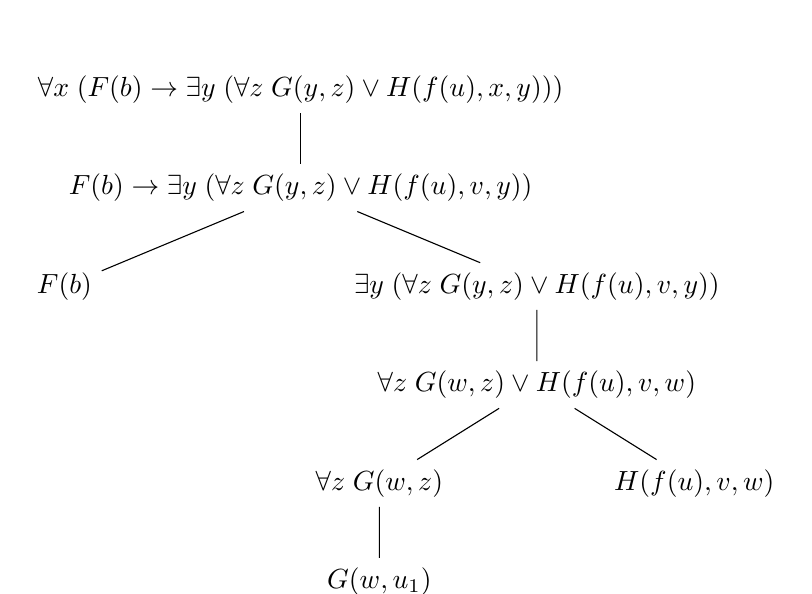
\begin{tikzpicture}[
  level distance=1.25cm,
  level 1/.style={sibling distance=3cm},
  level 2/.style={sibling distance=6cm},
  level 3/.style={sibling distance=3cm},
  level 4/.style={sibling distance=4cm},
  sibling distance=8cm,
  tlabel/.style={pos=0.4,right=-1pt,font=\footnotesize\color{black}},
  edge from parent path={(\tikzparentnode) -- (\tikzchildnode)}]
]
\node{$\forall x \; (F(b) \rightarrow \exists y \; (\forall z \; G(y, z) \vee H(f(u), x, y)))$}
child {node {$F(b) \rightarrow \exists y \; (\forall z \; G(y, z) \vee H(f(u), v, y))$}
  child {node {$F(b)$}}
  child {node {$\exists y \; (\forall z \; G(y, z) \vee H(f(u), v, y))$}
    child {node {$\forall z \; G(w, z) \vee H(f(u), v, w)$}
      child {node {$\forall z \; G(w, z)$}
         child {node {$G(w, u_1)$}}
      }
      child {node {$H(f(u), v, w)$}}
    }
  }
};
\end{tikzpicture}
\end{center}
\end{exmp}

\newpage
\section{Semantics of Predicate Logic}

In propositional logic, we need a truth valuation to give meaning to a formula.

In predicate logic, we need a valuation to give a meaning to a term or formula.

\subsection{Valuation}

\begin{defn}[Valuation]
A valuation $v$ for our language $\mathcal{L}$ consists of:\vspace{-0.25cm}
\begin{enumerate}
    \item a domain $\mathcal{D}$
    \item a meaning for each individual symbol (e.g. $a^v \in \mathcal{D}$)
    \item a meaning for each free variable symbol (e.g. $u^v \in \mathcal{D}$)
    \item a meaning for each relation symbol (e.g. $F^v \subseteq \mathcal{D}^n$, $\approx^v = \{\langle x, x \rangle \mid x \in \mathcal{D}\} \subseteq \mathcal{D}^2$)
    \item a meaning for each function symbol (e.g. $f^v : \mathcal{D}^m \to \mathcal{D}$)
\end{enumerate}
\end{defn}

A function symbol $f$ must be interpreted as a function $f^v$ that is total on the domain $\mathcal{D}$.
$$f^v : \mathcal{D}^m \to \mathcal{D}$$
Any $m$-tuple $(d_1, \dots, d_m) \in \mathcal{D}^m$ can be an input to $f^v$.

For any legal $m$-tuple $(d_1, \dots, d_m) \in \mathcal{D}^m$, it follows that $f^v (d_1^v, \dots, d_m^v) \in \mathcal{D}$.

\subsection{Value of Terms}
\begin{defn}[Value of Terms]
The value of terms of $\mathcal{L}$ under valuation $v$ over the domain $\mathcal{D}$ is defined by recursion:\vspace{-0.25cm}
\begin{enumerate}
    \item $a^v \in \mathcal{D}$
    \item $u^v \in \mathcal{D}$
    \item $f(t_1, \dots, t_n)^v = f^v(t_1^v, \dots, t_n^v)$
\end{enumerate}
\end{defn}

\subsection{Truth Value of Formulas}

The assignment override notation: $v(u/\alpha)$ keeps all the mappings in $v$ intact {\it except} reassigning $u$ to $\alpha \in \mathcal{D}$.

\begin{defn}[Truth Value of Formulas]
The truth value of formulas of $\mathcal{L}$ under valuation $v$ over domain $\mathcal{D}$ is defined by recursion:\vspace{-0.25cm}
\begin{enumerate}
    \item $F(t_1, \dots, t_n)^v = 1$ if and only if $\langle t_1^v, \dots, t_n^v \rangle \in F^v$. 
    
    {\bf Example of this notation:} \\ 
    Let $F^v = \{ \langle 1, 1 \rangle, \langle 2, 3 \rangle \}$. Then $F(1, 1) = 1$, $F(2, 3) = 1$, $F(2, 1) = 0$, and $F(3, 3) = 0$.
    \item $(\neg A)^v = 1$ if and only if $A^v = 0$.
    \item $(A \wedge B)^v = 1$ if and only if $A^v = 1$ and $B^v = 1$.
    \item $(A \vee B)^v = 1$ if and only if $A^v = 1$ or $B^v = 1$.
    \item $(A \rightarrow B)^v = 1$ if and only if $A^v = 0$ or $B^v = 1$.
    \item $(A \leftrightarrow B)^t = 1$ if and only if $A^v = B^v$.
    \item $(\forall x \; A(x))^v = 1$ if and only if for every $\alpha \in \mathcal{D}$, $A(u)^{v(u/\alpha)} = 1$, where $u$ does not occur in $A(x)$.
    \item $(\exists x \; A(x))^v = 1$ if and only if there exists $\alpha \in \mathcal{D}$ such that $A(u)^{v(u/\alpha)} = 1$, where $u$ does not occur in $A(x)$.
\end{enumerate}
\end{defn}

\subsection{Satisfiable and Valid}
A formula $A$ is {\bf satisfiable} if there exists a valuation $v$ such that $A^v = 1$.

A formula $A$ is {\bf valid} if for every valuation $v$, $A^v = 1$.

Valid corresponds to a tautology, unsatisfiable corresponds to a contradiction, and any other formula is satisfiable but not valid.

\begin{exmp}
Is the following formula satisfiable? If it is satisfiable, give a valuation that satisfies it. If it is not satisfiable, give a proof.
$$(\exists x \; F(x)) \rightarrow (\forall x \; F(x))$$
This formula is satisfiable.

Consider the valuation $v$ such that the domain is $\mathcal{D} = \{1\}$ and $F^v = \varnothing$. 

Since $F^v = \varnothing$, $F(u)^{v(u/\alpha)} = 0$ for every $\alpha \in \mathcal{D}$. Thus, $(\exists x \; F(x))^v = 0$, and it follows that $((\exists x \; F(x)) \rightarrow (\forall x \; F(x)))^v = 1$.

(Alternatively, $F^v = \{1\}$ works as well.)
\end{exmp}

\begin{exmp}
Is the following formula valid? If it is valid, give a proof. If it is not valid, give a counterexample.
$$(\forall x \; F(x)) \rightarrow (\exists x \; F(x))$$
This formula is valid.

\begin{pf}
We prove this by contradiction. Assume that there exists a valuation $v$ such that $(\forall x \; F(x))^v = 1$ and $(\exists x \; F(x))^v = 0$.

Since $(\forall x \; F(x))^v = 1$, we have that:
$$\text{For every $\alpha \in \mathcal{D}$, $F(u)^{v(u/\alpha)} = 1$} \quad (*)$$
Since $(\exists x \; F(x))^v = 0$, then:
$$\text{There exists $\beta \in \mathcal{D}$, $F(u)^{v(u/\beta)} = 0$} \quad (**)$$
($**$) is a contradiction with $(*)$. Thus, the formula must be valid.
\end{pf}
\end{exmp} 

\begin{exmp}
Is the following formula valid? If it is valid, give a proof. If it is not valid, give a counterexample.
$$(\exists x \; F(x)) \rightarrow (\forall x \; F(x))$$
This formula is not valid.

Consider the valuation $v$ such that the domain is $\mathcal{D} = \{1, 2\}$ and $F^v = \{1\}$. 

Since $1 \in F^v$, $F(u)^{v(u/1)} = 1$. Thus, $(\exists x \; F(x))^v = 1$.

Since $2 \notin F^v$, $F(u)^{v(u/2)} = 0$. Thus, $(\forall x \; F(x))^v = 0$. 
\end{exmp}

\begin{remark}
There is no way of enumerating all the valuations, so a truth table is not a valid proof method in predicate logic.
\end{remark}

\newpage
\section{Logical Consequence}

\subsection{Definition of Logical Consequence}
Define the symbols:\vspace{-0.25cm}
\begin{itemize}
    \item $\Sigma$ is a set of predicate formulas.
    \item $A$ is a predicate formula.
\end{itemize}

\begin{defn}
We say that $\Sigma$ {\bf logically implies} $A$, or $A$ is a logical consequence of $\Sigma$, if and only if for every valuation $v$, $\Sigma^v = 1$ implies $A^v = 1$. This is denoted $\Sigma \vDash A$.
\end{defn}

\subsection{Proving or Disproving a Logical Consequence}
\begin{exmp}
Consider the logical consequence below.
$$\forall x \; \neg A(x) \vDash \neg(\exists x \; A(x))$$
If the logical consequence holds, prove it. Otherwise, provide a counterexample.

The logical consequence holds.

\begin{pf}
We prove this by contradiction. Assume that there exists a valuation $v$ such that $(\forall x \; \neg A(x))^v = 1$ and $\neg (\exists x \; A(x))^v = 0$. 

Since $(\forall x \; \neg A(x))^v = 1$, $(\neg A(u))^{v(u/\alpha)} = 1$ for every $\alpha \in \mathcal{D}$. Hence, 
$$A(u)^{v(u/\alpha)} = 0 \text{ for every } \alpha \in \mathcal{D}. \quad (*)$$
Since $(\neg (\exists x \; A(x)))^v = 0$, we have $(\exists x \; A(x))^v = 1$. Then
$$A(u)^{v(u/\beta)} = 1 \text{ for some } \beta \in \mathcal{D} \quad (**)$$
($**$) contradicts ($*$), thus the logical consequence holds.
\end{pf}
\end{exmp}

\begin{exmp}
Consider the logical consequence below.
$$\forall x \; (A(x) \rightarrow B(x)) \vDash \forall x \; A(x) \rightarrow \forall x \; B(x)$$
If the logical consequence holds, prove it. Otherwise, provide a counterexample.

The logical consequence holds.

\begin{pf}
We prove by contradiction. Assume that there exists a valuation $v$ such that
\begin{equation}
    (\forall x \; (A(x) \rightarrow B(x)))^v = 1
\end{equation}
and such that
\begin{equation}
    ((\forall x \; A(x)) \rightarrow (\forall x \; B(x)))^v = 0
\end{equation}
By (2), we obtain
\begin{align}
    (\forall x \; A(x))^v &= 1 \\
    (\exists x \; B(x))^v &= 0
\end{align}
By (3), 
\begin{equation}
    A(u)^{v(u/\alpha)} = 1 \text{ for every } \alpha \in \mathcal{D}
\end{equation}
By (4),
\begin{equation}
    B(u)^{v(u/\beta)} = 0 \text{ for some } \beta \in \mathcal{D}
\end{equation}
By (1), 
\begin{equation}
    (A(u) \rightarrow B(u))^{v(u/\alpha)} = 1 \text{ for every } \alpha \in \mathcal{D}
\end{equation}
By (5) and (6), $A(u)^{v(u/\beta)} = 1$ and $B(u)^{v(u/\beta)} = 0$. Thus $(A(u) \rightarrow B(u))^{v(u/\beta)} = 0$, which contradicts (7). Hence, the logical consequence must hold.
\end{pf}
\end{exmp}

\begin{exmp}
Consider the logical consequence below.
$$\forall x \; A(x) \rightarrow \forall x \; B(x) \vDash \forall x \; (A(x) \rightarrow B(x))$$
If the logical consequence holds, prove it. Otherwise, provide a counterexample.

Consider the valuation $v$ such that the domain is $\mathcal{D} = \{1, 2\}$, $A^v = 1$, and $B^v = \varnothing$. 
\end{exmp}

\newpage
\section{Formal Deduction in Predicate Logic}

\subsection{$\forall$-elimination ($\forall-$)}
\vspace{-0.25cm}
\begin{align*}
    \text{if } \Sigma &\vdash \forall x \, A(x), \\
    \text{then } \Sigma &\vdash A(t).
\end{align*}
($\forall-$) is analogous to $(\wedge-)$.

\begin{exmp}
Show that $\{P(u), \forall x \, (P(x) \rightarrow (\neg Q(x)))\} \vdash \neg Q(u)$.
\begin{align*}
    (1) & & P(u),\, \forall x \, (P(x) \rightarrow \neg Q(x)) &\vdash \forall x \, (P(x) \rightarrow \neg Q(x)) & & \text{by ($\in$)} \\
    (2) & & P(u),\, \forall x \, (P(x) \rightarrow \neg Q(x)) &\vdash P(u) \rightarrow \neg Q(u) & & \text{by ($\forall-$, 1)} \\
    (3) & & P(u),\, \forall x \, (P(x) \rightarrow \neg Q(x)) &\vdash P(u) & & \text{by ($\in$)} \\
    (4) & & P(u),\, \forall x \, (P(x) \rightarrow \neg Q(x)) &\vdash \neg Q(u) & & \text{by ($\rightarrow-$, 2, 3)} 
\end{align*}
\end{exmp}

\subsection{$\exists$-introduction ($\exists+$)}
\vspace{-0.25cm}
\begin{align*}
    \text{if } \Sigma &\vdash A(t), \\
    \text{then } \Sigma &\vdash \exists x \, A(x).
\end{align*}
($\exists+$) is analogous to ($\vee+$). $A(x)$ comes from replacing some (not necessarily all) occurrences of $t$ in $A(t)$ by $x$.


\begin{exmp}
Show that $\{\neg P(v)\} \vdash \exists x\,(P(x) \rightarrow Q(x))$.
\begin{align*}
    (1) & & \neg P(v),\, P(v),\, \neg Q(v) &\vdash \neg P(v) & & \text{by ($\in$)} \\
    (2) & & \neg P(v),\, P(v),\, \neg Q(v) &\vdash P(v) & & \text{by ($\in$)} \\
    (3) & & \neg P(v),\, P(v) &\vdash Q(v) & & \text{by ($\neg-$, 1, 2)} \\
    (4) & & \neg P(v) &\vdash P(v) \rightarrow Q(v) & & \text{by ($\rightarrow+$, 3)} \\
    (5) & & \neg P(v) &\vdash \exists x\,(P(x) \rightarrow Q(x)) & & \text{by ($\exists+$, 4)}
\end{align*}
\end{exmp}

\subsection{$\forall$-introduction ($\forall+$)}
\vspace{-0.25cm}
\begin{align*}
    \text{if } \Sigma &\vdash A(u),\, u \text{ not occurring in $\Sigma$,} \\
    \text{then } \Sigma &\vdash \forall x \, A(x).
\end{align*}
($\forall+$) is analogous to ($\wedge+$). This requires $u$ to be an arbitrary element. This means that the choice of $u$ is independent of the premises of $\Sigma$. If $u$ has a certain property, the conclusion may not be valid.

\begin{exmp}
Show that $\{\forall x\,(P(x) \rightarrow Q(x))\} \vdash (\forall x \, P(x)) \rightarrow (\forall y \, Q(y))$.
\begin{align*}
    (1) & & \forall x\,(P(x) \rightarrow Q(x)),\, \forall x \, P(x) &\vdash \forall x\,(P(x) \rightarrow Q(x)) & & \text{by ($\in$)} \\
    (2) & & \forall x\,(P(x) \rightarrow Q(x)),\, \forall x \, P(x) &\vdash P(u) \rightarrow Q(u) & & \text{by ($\forall-$, 1)} \\
    (3) & & \forall x\,(P(x) \rightarrow Q(x)),\, \forall x \, P(x) &\vdash \forall x \, P(x) & & \text{by ($\in$)} \\
    (4) & & \forall x\,(P(x) \rightarrow Q(x)),\, \forall x \, P(x) &\vdash P(u) & & \text{by ($\forall-$, 3)} \\
    (5) & & \forall x\,(P(x) \rightarrow Q(x)),\, \forall x \, P(x) &\vdash Q(u) & & \text{by ($\rightarrow-$, 2, 4)} \\
    (6) & & \forall x\,(P(x) \rightarrow Q(x)),\, \forall x \, P(x) &\vdash \forall y \, Q(y) & & \text{by ($\forall+$, 5)} \\
    (7) & & \forall x\,(P(x) \rightarrow Q(x)) &\vdash (\forall x \, P(x)) \rightarrow (\forall y \, Q(y)) & & \text{by ($\rightarrow+$, 6)}
\end{align*}
\end{exmp}

\subsection{$\exists$-elimination ($\exists-$)}
\vspace{-0.25cm}
\begin{align*}
    \text{if } \Sigma,\, A(u) &\vdash B,\, u \text{ not occurring in $\Sigma$ or $B$} \\
    \text{then } \Sigma,\, \exists x\,A(x) &\vdash B.
\end{align*}
($\exists-$) is analogous to ($\vee-$). A way to think about this rule is proof by cases. The conclusion may have nothing to do with the starting formula.

\begin{exmp}
Show that $\{\exists x \, (P(x) \vee Q(x))\} \vdash (\exists x \, P(x)) \vee (\exists x \, Q(x))$.
\begin{align*}
    (1) & & P(u) &\vdash P(u) & & \text{by ($\in$)} \\
    (2) & & Q(u) &\vdash Q(u) & & \text{by ($\in$)} \\
    (3) & & P(u) &\vdash \exists x \, P(x) & & \text{by ($\exists+$, 1)} \\
    (4) & & Q(u) &\vdash \exists x \, Q(x) & & \text{by ($\exists+$, 2)} \\
    (5) & & P(u) &\vdash (\exists x \, P(x)) \vee (\exists x \, Q(x)) & & \text{by ($\vee+$, 3)} \\
    (6) & & Q(u) &\vdash (\exists x \, P(x)) \vee (\exists x \, Q(x)) & & \text{by ($\vee+$, 4)} \\
    (7) & & P(u) \vee Q(u) &\vdash (\exists x \, P(x)) \vee (\exists x \, Q(x)) & & \text{by ($\vee-$, 5, 6)} \\
    (8) & & \exists x \, (P(x) \vee Q(x)) &\vdash (\exists x \, P(x)) \vee (\exists x \, Q(x)) & & \text{by ($\exists-$, 6)}
\end{align*}
\end{exmp}

\newpage
\section{Soundness and Completeness of Formal Deduction}

\subsection{Soundness and Completeness}
Soundness: $\Sigma \vdash A \rightarrow \Sigma \vDash A$.

Completeness: $\Sigma \vDash A \rightarrow \Sigma \vdash A$.

\subsection{Proving Inference Rules are Sound}
\begin{thm}
The $\forall-$ inference rule is sound. That is, if $\Sigma \vDash \forall x \, A(x)$, then $\Sigma \vDash A(t)$, where $t$ is a term.

\begin{pf}
Assume that $\Sigma \vDash \forall x \, A(x)$ holds. We need to show that $\Sigma \vDash A(t)$, where $t$ is a term. (That is, for every valuation $v$, $\Sigma^v = 1$ implies that $A(t)^v = 1$.) 

Consider an arbitrary valuation $v$ such that $\Sigma^v = 1$.

We know that $\Sigma \vDash \forall x \, A(x)$ and $\Sigma^v = 1$, so we obtain $(\forall x \ A(x))^v = 1$. 

By the semantics of $\forall$,
$$A(u)^{v(u/\alpha)} = 1 \text{ for every } \alpha \in \mathcal{D} \quad (*)$$
We have the following two facts:

{\sc Fact 1.} Since $t$ is a term, $t^v \in \mathcal{D}$ (exercise: structural induction on terms).

{\sc Fact 2.} We have $A(t)^v = A(u)^{v(u/t^v)}$ (exercise).

Then by ($*$), Fact 1, and Fact 2, we obtain
$$A(t)^v = A(u)^{v(u/t^v)} = 1$$
Hence $\Sigma \vDash A(t)$, as required.
\end{pf}
\end{thm}

\begin{thm}
The $\exists-$ inference rule is sound. That is, if $\Sigma,\, A(u) \vDash B$, where $u$ does not occur in $\Sigma$ or $B$, then $\Sigma,\, (\exists x\, A(x)) \vDash B$.
\begin{pf}
Assume that $\Sigma,\, A(u) \vDash B$, where $u$ does not occur in $\Sigma$ or $B$.

Consider an arbitrary valuation $v$ such that $\Sigma^v = 1$ and $(\exists x\,A(x))^v = 1$. We show that $B^v = 1$.

Since $(\exists x\, A(x))^v = 1$, we have $A(u)^{v(u/\alpha)} = 1$ for some $\alpha \in \mathcal{D}$. 

Since $u$ does not occur in $\Sigma$, 
$$\Sigma^{v(u/\alpha)} = \Sigma^v = 1$$

We have $\Sigma,\, A(u) \vDash B$, and $u$ does not occur in $B$, thus
$$B^v = B^{v(u/\alpha)} = 1$$
Hence $\Sigma,\, (\exists x\, A(x)) \vDash B$ holds.
\end{pf}
\end{thm}

\newpage
\section{Peano Arithmetic}

\subsection{Formal Deduction Rules for Equality}
\vspace{-0.25cm}
\begin{align*}
(\approx-) \quad &\text{If $\Sigma \vdash A(t_1)$ and $\Sigma \vdash t_1 \approx t_2$, then} \\ &\text{$\Sigma \vdash A'(t_2)$,} \\ &\text{where $A'(t_2)$ results from $A(t_1)$} \\ &\text{by replacing some (not necessarily all) occurrences} \\ &\text{of $t_1$ by $t_2$.} \\\\
(\approx+) \quad &\varnothing \vdash u \approx u
\end{align*}

\subsection{Reflexivity, Symmetry, Transitivity}
{\bf Reflexivity:} $\varnothing \vdash \forall x \, (x \approx x)$
\begin{align*}
    &(1) & \varnothing &\vdash u \approx u & & \text{by ($\approx+$)} \\
    &(2) & \varnothing &\vdash \forall x \, (x \approx x) & & \text{by ($\forall+$, 1)}
\end{align*}
{\bf Symmetry:} $\varnothing \vdash \forall x \, \forall y \, (x \approx y) \to (y \approx x)$
\begin{align*}
    &(1) & \varnothing &\vdash u \approx u & & \text{by ($\approx+$)} \\
    &(2) & u \approx v &\vdash u \approx u & & \text{by ($+$, 1)} \\
    &(3) & u \approx v &\vdash u \approx v & & \text{by ($\in$)} \\
    &(4) & u \approx v &\vdash v \approx u & & \text{by ($\approx-$, 2, 3)} \\
    &(5) & \varnothing &\vdash (u \approx v) \to (v \approx u) & & \text{by ($\rightarrow+$, 4)} \\
    &(6) & \varnothing &\vdash \forall y \, (u \approx y) \to (y \approx u) & & \text{by ($\forall+$, 5)} \\
    &(7) & \varnothing &\vdash \forall x \, \forall y \, (x \approx y) \to (y \approx x) & & \text{by ($\forall+$, 6)}
\end{align*}
When using ($\approx-$), we had $t_1 = u$, $t_2 = v$, and $A(x) = x \approx u$.

{\bf Transitivity:} $\varnothing \vdash \forall x \, \forall y \, \forall z \, (x \approx y) \wedge (y \approx z) \to (x \approx z)$
\begin{align*}
    &(1) & (u \approx v) \wedge (v \approx w) &\vdash (u \approx v) \wedge (v \approx w) & & \text{by ($\in$)} \\
    &(2) & (u \approx v) \wedge (v \approx w) &\vdash u \approx v & & \text{by ($\wedge-$, 1)} \\
    &(3) & (u \approx v) \wedge (v \approx w) &\vdash v \approx w & & \text{by ($\wedge-$, 1)} \\
    &(4) & (u \approx v) \wedge (v \approx w) &\vdash u \approx w & & \text{by ($\approx-$, 2, 3)} \\
    &(5) & \varnothing &\vdash (u \approx v) \wedge (v \approx w) \to (u \approx w) & & \text{by ($\rightarrow+$, 4)} \\
    &(6) & \varnothing &\vdash \forall z \, (u \approx v) \wedge (v \approx z) \to (u \approx z) & & \text{by ($\forall+$, 5)} \\
    &(7) & \varnothing &\vdash \forall y \, \forall z \, (u \approx y) \wedge (y \approx z) \to (u \approx z) & & \text{by ($\forall+$, 6)} \\
    &(8) & \varnothing &\vdash \forall x \, \forall y \, \forall z \, (x \approx y) \wedge (y \approx z) \to (x \approx z) & & \text{by ($\forall+$, 7)}
\end{align*}
When using ($\approx-$), we had $t_1 = v$, $t_2 = w$, and $A(x) = u \approx x$.

\subsection{Symbols for Number Theory}
Individual symbol (or constant): 0 

Functions: addition ($+$), multiplication ($\cdot$), successor ($s(x)$)

In this way, we can write $s(0) = 1$, $s(s(0)) = 2$, and so on.

\subsection{Peano Axioms}
Axioms for successor:\vspace{-0.25cm}
\begin{itemize}[label={}]
\item {\bf PA1} Zero is not a successor of any natural number. $$\forall x \, \neg(s(x) \approx 0)$$
\item {\bf PA2} If the successors of two numbers are the same, then the two numbers are the same.
$$\forall x \, \forall y \, (s(x) \approx s(y) \to x \approx y)$$
\end{itemize}
\vspace{-0.25cm}
Axioms for addition:\vspace{-0.25cm}
\begin{itemize}[label={}]
\item {\bf PA3} Adding zero to any number yields the same number.
$$\forall x \, (x + 0 \approx x)$$
\item {\bf PA4} Adding the successor of a number yields the successor of adding the number.
$$\forall x \, \forall y \, (x + s(y) \approx s(x+y))$$
\end{itemize}
\vspace{-0.25cm}
Axioms for multiplication:\vspace{-0.25cm}
\begin{itemize}[label={}]
\item {\bf PA5} Multiplying a number by zero yields zero.
$$\forall x \, (x \cdot 0 \approx 0)$$
\item {\bf PA6} Multiplying one number and the successor of another number equals the product of the two numbers plus the first number.
$$\forall x \, \forall y \, (x \cdot s(y) \approx x \cdot y + x)$$
\end{itemize}
Axiom for induction:\vspace{-0.25cm}
\begin{itemize}[label={}]
\item {\bf PA7} For each predicate formula $A(x)$ with free variable $x$, we have
$$(A(0) \wedge \forall x \, (A(x) \to A(s(x)))) \to \forall x \, A(x)$$
\end{itemize}

\newpage
\subsection{Induction on the Natural Numbers}
\begin{exmp}
Prove that $\forall x \, (\neg (s(x) \approx x))$.
\begin{align*}
    &(1) & \varnothing &\vdash \forall x \, (\neg (s(x) \approx 0)) & & \text{by (PA1)} \\
    &(2) & \varnothing &\vdash \neg(s(0) \approx 0) & & \text{by ($\forall-$, 1)} \\
    &(3) & \varnothing &\vdash \forall x \, \forall y \, s(x) \approx s(y) \to x \approx y & & \text{by (PA2)} \\
    &(4) & \varnothing &\vdash \forall y \, s(s(u)) \approx s(y) \to s(u) \approx y & & \text{by ($\forall-$, 3)} \\
    &(5) & \varnothing &\vdash s(s(u)) \approx s(u) \to s(u) \approx u & & \text{by ($\forall-$, 4)} \\
    &(6) & \neg (s(u) \approx u),\, s(s(u)) \approx s(u) &\vdash s(s(u)) \approx s(u) \to s(u) \approx u & & \text{by ($+$, 5)} \\
    &(7) & \neg (s(u) \approx u),\, s(s(u)) \approx s(u) &\vdash s(s(u)) \approx s(u) & & \text{by ($\in$)} \\
    &(8) & \neg (s(u) \approx u),\, s(s(u)) \approx s(u) &\vdash s(u) \approx u & & \text{by ($\to-$, 6, 7)} \\
    &(9) & \neg (s(u) \approx u),\, s(s(u)) \approx s(u) &\vdash \neg (s(u) \approx u) & & \text{by ($\in$)} \\
    &(10) & \neg (s(u) \approx u) &\vdash \neg(s(s(u)) \approx s(u)) & & \text{by ($\neg+$, 8, 9)} \\
    &(11) & \varnothing &\vdash \neg (s(u) \approx u) \to \neg(s(s(u)) \approx s(u)) & & \text{by ($\rightarrow-$, 10)} \\
    &(12) & \varnothing &\vdash \forall x \, (\neg (s(x) \approx x) \to \neg(s(s(x)) \approx s(x))) & & \text{by ($\forall+$, 11)} \\
    &(13) & \varnothing &\vdash \neg(s(0) \approx 0) \wedge \forall x \, (\neg (s(x) \approx x) \\ &&& \qquad\qquad \to \neg(s(s(x)) \approx s(x))) & & \text{by ($\wedge+$, 2, 12)} \\
    &(14) & \varnothing &\vdash (\neg (s(0) \approx 0) \wedge \forall x \, (\neg (s(x) \approx x) \\ &&& \qquad\qquad \to \neg (s(s(x)) \approx s(x)))) \\ &&& \qquad\qquad \to \forall x \, (\neg (s(x) \approx x)) & & \text{by (PA7)} \\
    &(15) & \varnothing &\vdash \forall x \, (\neg (s(x) \approx x)) & & \text{by ($\to-$, 13, 14)}
\end{align*}
\end{exmp}

\begin{exmp}
Prove that $\forall x \, (x \approx 0 \vee \exists y \, (s(y) \approx x))$. 
\begin{align*}
    &(1) & \varnothing &\vdash 0 \approx 0 & & \text{by ($\approx+$)} \\
    &(2) & \varnothing &\vdash 0 \approx 0 \vee \exists y \, (s(y) \approx 0) & & \text{by ($\forall+$, 1)} \\
    &() & \varnothing &\vdash \forall x \, (x \approx 0 \vee \exists y \, (s(y) \approx x) \rightarrow s(x) \approx 0 \vee \exists y \, (s(y) \approx s(x))) & & \text{by ()} \\
    &&& \text{prove induction step (the one above)} \\
    &() & \varnothing &\vdash 0 \approx 0 \vee \exists y \, (s(y) \approx 0)) \wedge \forall x \, (x \approx 0 \vee \exists y \, (s(y) \approx x) \\ &&& \qquad\qquad \to s(x) \approx 0 \vee \exists y \, (s(y) \approx s(x))) & & \text{by ($\wedge+$, 2,)} \\
    &() & \varnothing &\vdash (0 \approx 0 \vee \exists y \, (s(y) \approx 0)) \wedge \forall x \, (x \approx 0 \vee \exists y \, (s(y) \approx x) \\ &&& \qquad\qquad \to s(x) \approx 0 \vee \exists y \, (s(y) \approx s(x))) \\ &&& \qquad\qquad \to \forall x \, (x \approx 0 \vee \exists y \, (s(y) \approx x)) & & \text{by (PA7)} \\
    &() & \varnothing &\vdash \forall x \, (x \approx 0 \vee \exists y \, (s(y) \approx x)) & & \text{by ($\to-$)}
\end{align*}
\end{exmp}

\newpage
\section{Introduction to Undecidability}
\subsection{Decision Problems are Decidable or Undecidable}
A {\bf decision problem} is a problem which calls for an answer of yes or no, given some input.

A decision problem is {\bf decidable} if and only if there exists an algorithm that produces the correct output for the problem for every input. Otherwise, the decision problem is {\bf undecidable}.

\begin{remark} Some remarks about decidable and undecidable problems:\vspace{-1.5ex}
\begin{itemize}
    \item An algorithm must terminate after finitely many steps.
    \item To prove that a problem is decidable, we write down an algorithm to solve it for every input.
    \item For an undecidable problem, there may exist an algorithm which gives the correct output for the problem for some particular outputs. The problem is undecidable because no algorithm can give the correct output for the problem for every input.
\end{itemize}
\end{remark}

\subsection{The Halting Problem}
The decision problem: Given a program $P$ and an input $I$, will $P$ halt when run with input $I$?

This is one of the first known undecidable problems, called the Halting problem.

There does not exists an algorithm $H$ which gives the correct answer for the Halting problem, for every program $P$ and every input $I$.

Transforming this into a predicate formula, let:\vspace{-1.5ex}
\begin{itemize}
    \item $\mathcal{D} = \{\text{all algorithms, all programs, all inputs}\}$
    \item $A(x) : x$ is an algorithm
    \item $I(x) : x$ is an input
    \item $P(x) : x$ is a program
    \item $S(x, y, z) : x$ solves the Halting program for program $y$ and input $z$
\end{itemize}\vspace{-1.5ex}
Then we write
$$\neg (\exists x \, (A(x) \wedge \forall y \, \forall z \, (P(y) \wedge I(z) \rightarrow S(x, y, z))))$$
\begin{thm}
The Halting problem is undecidable.
\begin{pf}
Suppose to the contrary that there exists an algorithm $H(P, I)$ which gives the correct answer to the Halting problem for every program $P$ and every input $I$.

We construct an algorithm $X(P)$ which takes an program $P$ as input, and does the following things:\vspace{-1.5ex}
\begin{enumerate}[(1)]
\item Runs $H(P, P)$ (predicts whether $P$ will halt when run with input $P$).
\item If $H(P, P)$ outputs "yes", then $X$ does not halt. If $H(P, P)$ outputs "no", then $X$ halts.
\end{enumerate}\vspace{-1.5ex}
We claim that $H$ is always wrong when predicting whether $X$ halts when run with input $X$.

{\sc Case 1.} If $H(X, X)$ outputs "yes", then $H$ predicts that $X$ halts when run with input $X$. But $X$ does not halt when run with input $X$.

{\sc Case 2.} If $H(X, X)$ outputs "no", then $H$ predicts that $X$ does not halt when run with input $X$. But $X$ halts when run with input $X$.

In both cases, $H$ makes an incorrect prediction, which is a contradiction. Thus, there does not exist an algorithm that gives the correct answer to the Halting problem for every program $P$ and every input $I$, so the Halting problem is undecidable.
\end{pf}
\end{thm}

\newpage
\section{Proving Undecidability via Reductions}

\subsection{Idea of Reduction}
Reduce the halting problem to problem $P_B$.\vspace{-1.5ex}
\begin{itemize}
    \item Given an algorithm for solving $P_B$, we could use it to solve the halting problem.
    \item If $P_B$ is decidable, then the halting problem is decidable.
    \item If the halting problem is undecidable, then $P_B$ is undecidable.
\end{itemize}\vspace{-1.5ex}

\subsection{The {\tt HaltingNoInput} Problem}
The {\tt HaltingNoInput} problem: Given a program $P$ which takes no input, does $P$ halt?

\begin{thm}
The {\tt HaltingNoInput} problem is undecidable.
\begin{pf}
Suppose to the contrary that there exists an algorithm $B$ which solves the {\tt HaltingNoInput} problem.

Now, we construct an algorithm $A$:\vspace{-1.5ex}
\begin{itemize}
    \item $A$ takes two inputs: a program $P$ and an input $I$.
    \item Let program $P'$ run $P$ with input $I$, and return $P(I)$.
    \item Run algorithm $B$ with the program $P'$ as input.
    \item Return $B(P')$.
\end{itemize}\vspace{-1.5ex}
By the construction of algorithm $A$, we know that $P$ halts on input $I$ if and only if $P'$ halts.

Since algorithm $B$ solves the {\tt HaltingNoInput} problem, algorithm $A$ solves the halting problem, which contradicts the fact that the halting problem is undecidable. 

Thus, the {\tt HaltingNoInput} problem is undecidable. 
\end{pf}
\end{thm}

\subsection{The {\tt ExistsHaltingInput} Problem}
The {\tt ExistsHaltingInput} problem: Given a program $P$, does there exist an input $I$ such that $P$ halts with input $I$?
\begin{thm}
The {\tt ExistsHaltingInput} problem is undecidable.
\begin{pf}
Assume that there exists an algorithm $B$ which solves the {\tt ExistsHaltingInput} problem.

Construct an algorithm $A$ such that:\vspace{-1.5ex}
\begin{itemize}
    \item $A$ takes two inputs: a program $P$ and an input $I$.
    \item Let $P'$ be a program that ignores its input, runs $P$ with $I$, and returns $P(I)$.
    \item Run algorithm $B$ with $P'$ as its input.
    \item Return $B(P')$.
\end{itemize}\vspace{-1.5ex}
By our construction of algorithm $A$, we have that $P$ halts on input $I$ if and only if there exists an input $I'$ such that $P'$ halts on $I'$. 

Since algorithm $B$ solves the {\tt ExistsHaltingInput} problem, algorithm $A$ solves the halting problem, which contradicts the fact that the halting problem is undecidable.

Thus, the {\tt ExistsHaltingInput} problem is undecidable.
\end{pf}
\end{thm}

\end{document}